
%% %%
%% %% INTRO
%% %%


%% \slide{ Random notes }
%% {
%% \iteb
%% \item Mel Shochet (U. of C) and Peter Onyisi (Austin) added to the author list
%% \item Discovered that 0.2\% of data is missing in my ntuples (all in period-L)
%% \iteb
%% \item Re-making period-L right now. If it fails, may need to add a systematic
%% \item Recall that the current systematic on single-differential is about 1.0\%
%% \itee
%% \itee
%% }

%% %%
%% %% SMOOTHING SYSTEMATICS
%% %%

%% \slide{Smoothing systematics}
%% {
%% \centering
%% Smoothing parton shower and matrix element systematics, which suffer from low MC statistics

%% }

%% \slide{Parton Shower}
%% {
%%   \begin{itemize}
%%   \item Polynomial fits to the Parton Shower / Hadronization systematic
%%   \end{itemize}

%%   \begin{center}
%%     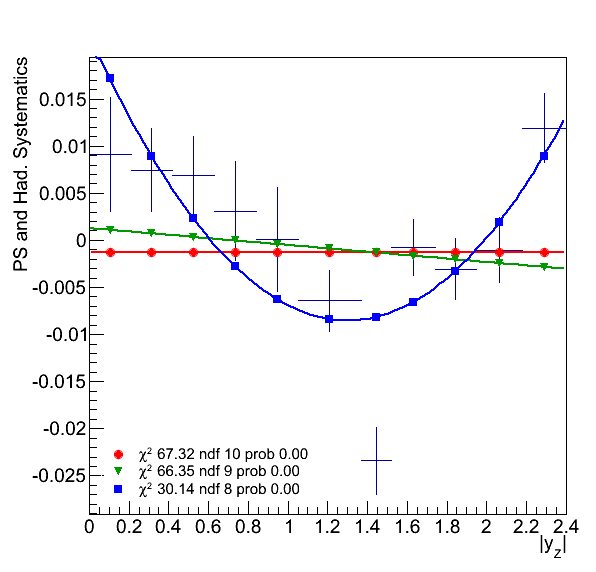
\includegraphics[width=0.3\textwidth]{dates/20130214/figures/smoothing/PSsyst_bin2.png}
%%     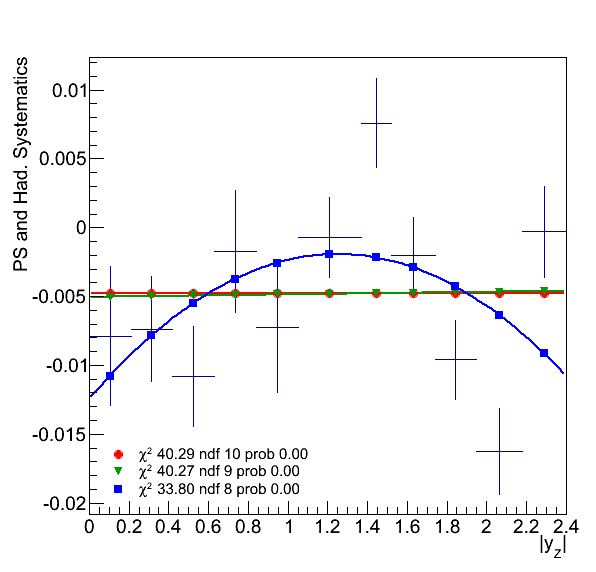
\includegraphics[width=0.3\textwidth]{dates/20130214/figures/smoothing/PSsyst_bin3.png}
%%     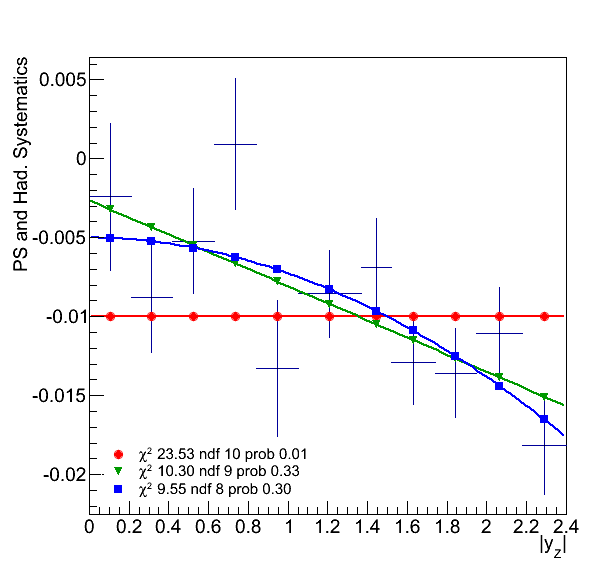
\includegraphics[width=0.3\textwidth]{dates/20130214/figures/smoothing/PSsyst_bin4.png}
%%   \end{center}

%%   \begin{center}
%%     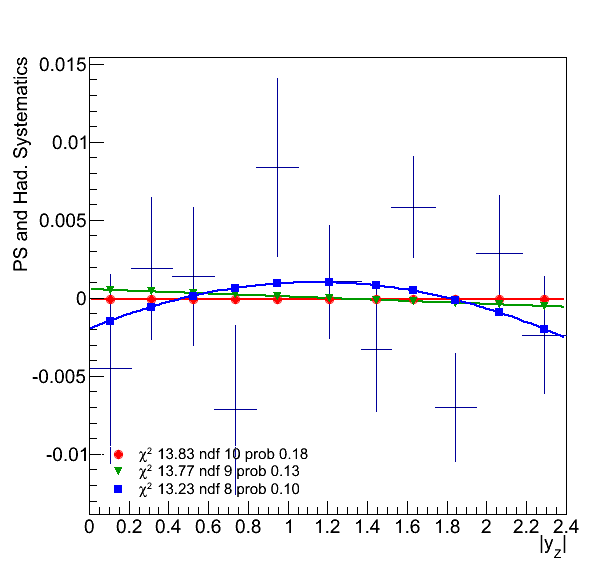
\includegraphics[width=0.3\textwidth]{dates/20130214/figures/smoothing/PSsyst_bin5.png}
%%     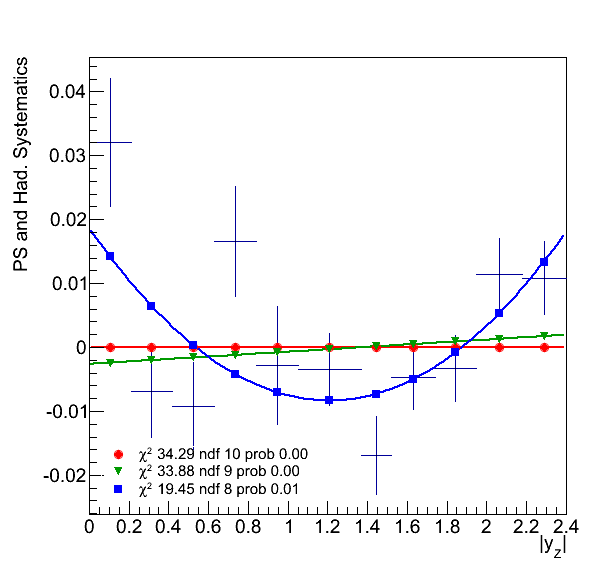
\includegraphics[width=0.3\textwidth]{dates/20130214/figures/smoothing/PSsyst_bin6.png}
%%     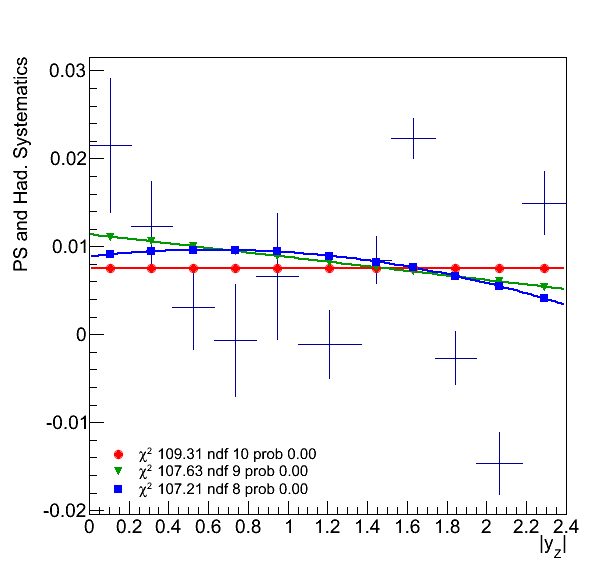
\includegraphics[width=0.3\textwidth]{dates/20130214/figures/smoothing/PSsyst_bin7.png}
%%   \end{center}

%% }

%% \slide{Matrix Element}
%% {
%%   \begin{itemize}
%%   \item Polynomial fits to the Matrix Element systematic
%%   \end{itemize}

%%   \begin{center}
%%     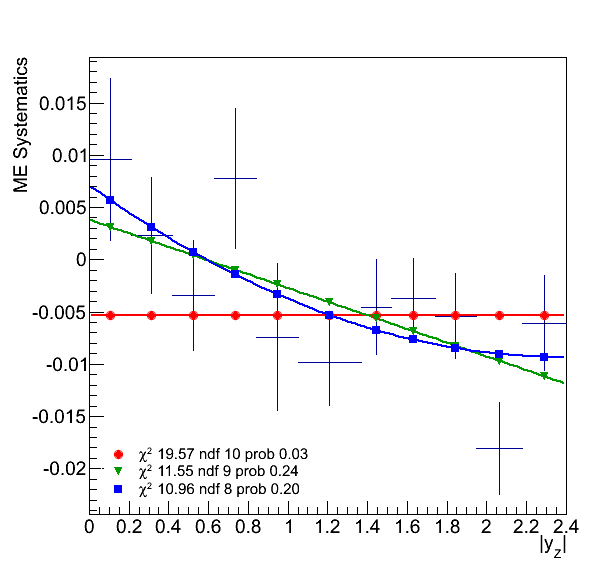
\includegraphics[width=0.3\textwidth]{dates/20130214/figures/smoothing/MEsyst_bin2.png}
%%     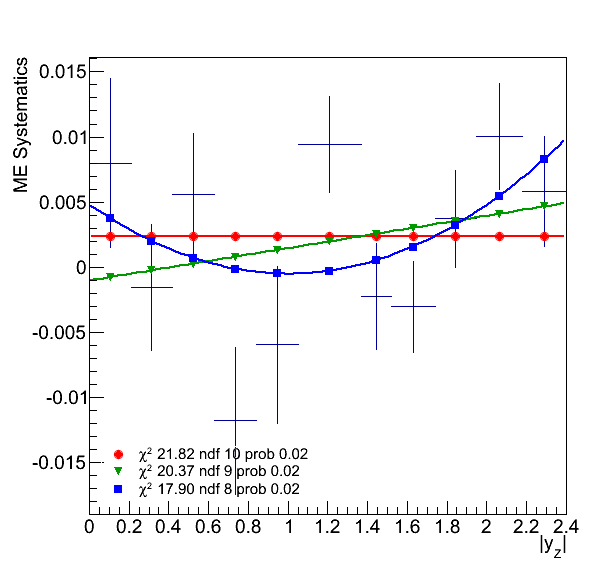
\includegraphics[width=0.3\textwidth]{dates/20130214/figures/smoothing/MEsyst_bin3.png}
%%     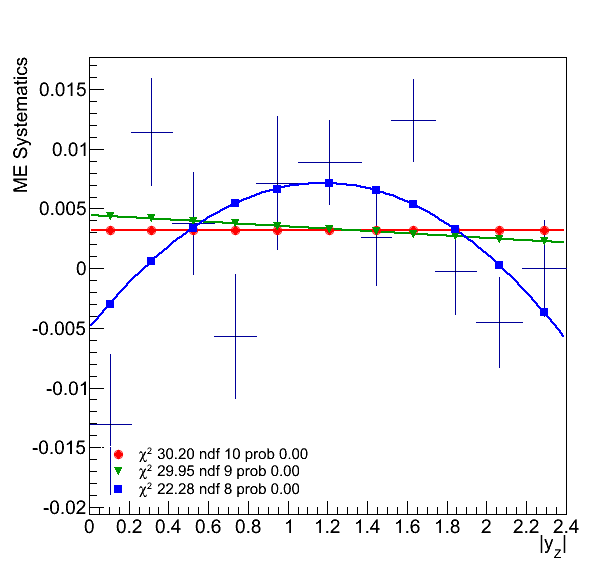
\includegraphics[width=0.3\textwidth]{dates/20130214/figures/smoothing/MEsyst_bin4.png}
%%   \end{center}

%%   \begin{center}
%%     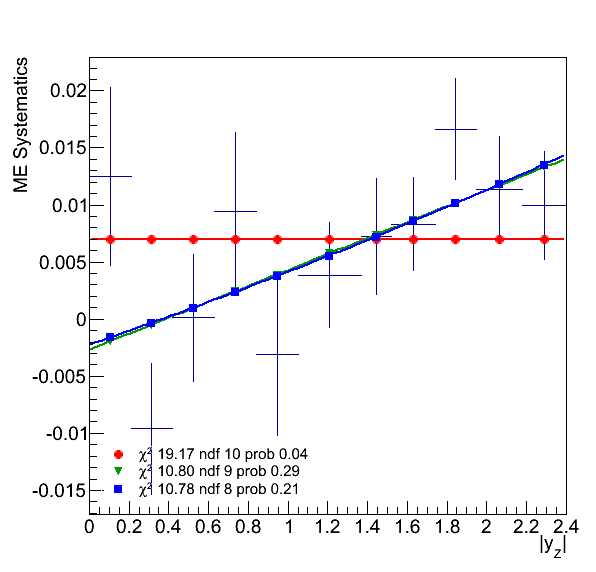
\includegraphics[width=0.3\textwidth]{dates/20130214/figures/smoothing/MEsyst_bin5.png}
%%     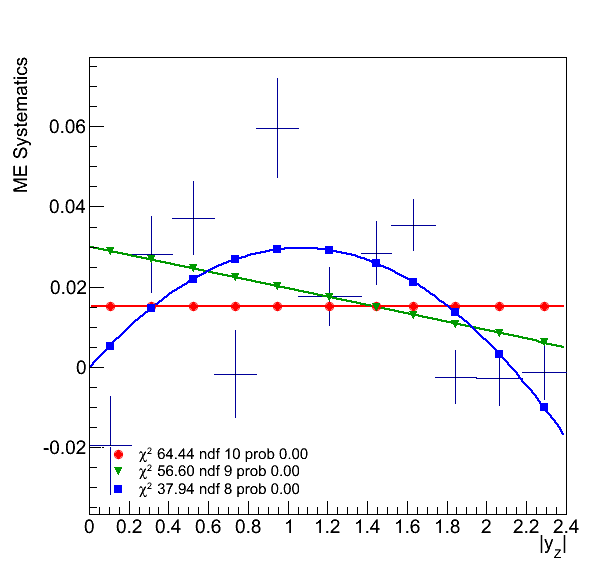
\includegraphics[width=0.3\textwidth]{dates/20130214/figures/smoothing/MEsyst_bin6.png}
%%     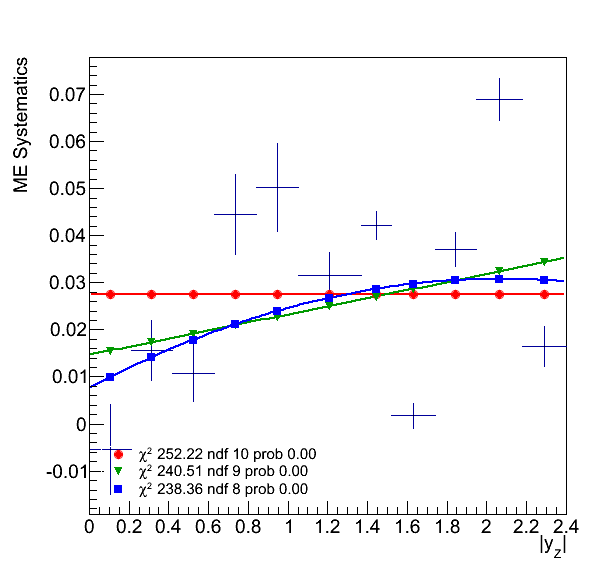
\includegraphics[width=0.3\textwidth]{dates/20130214/figures/smoothing/MEsyst_bin7.png}
%%   \end{center}

%% }

%% %%
%% %% FIRST E/MU COMPARISON PLOTS
%% %%

%% \slide{Electron-muon comparison}
%% {
%% \centering
%% \Huge First e/mu comparison plots

%% }

%% \slide{Single-differential W}
%% {
%% \colb[T]

%% \column{.5\textwidth}
%% \centering
%% \small{ $W^{+}$ }
%% 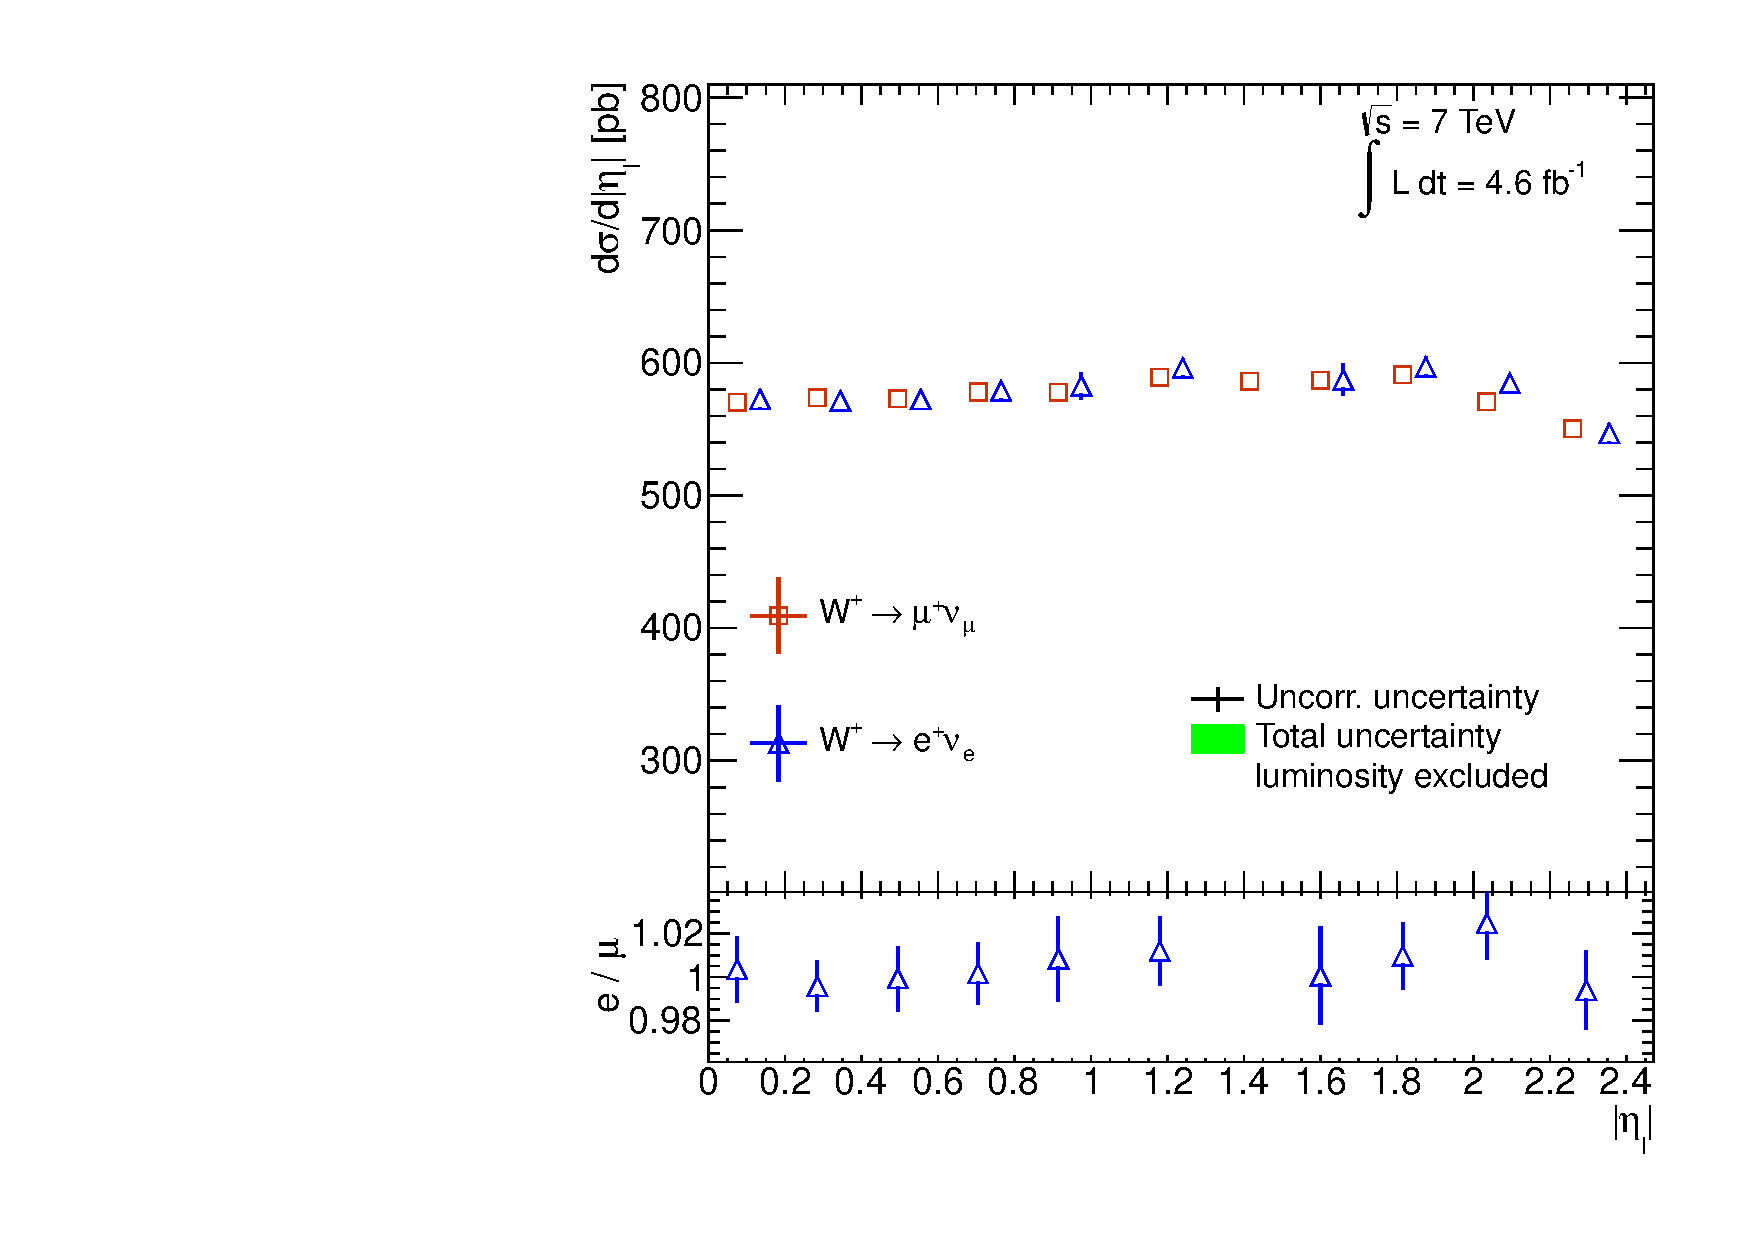
\includegraphics[width=1.0\textwidth]{dates/20130214/figures/plots/WPeta25_combined}

%% \column{.5\textwidth}
%% \centering
%% \small{ $W^{-}$ }
%% 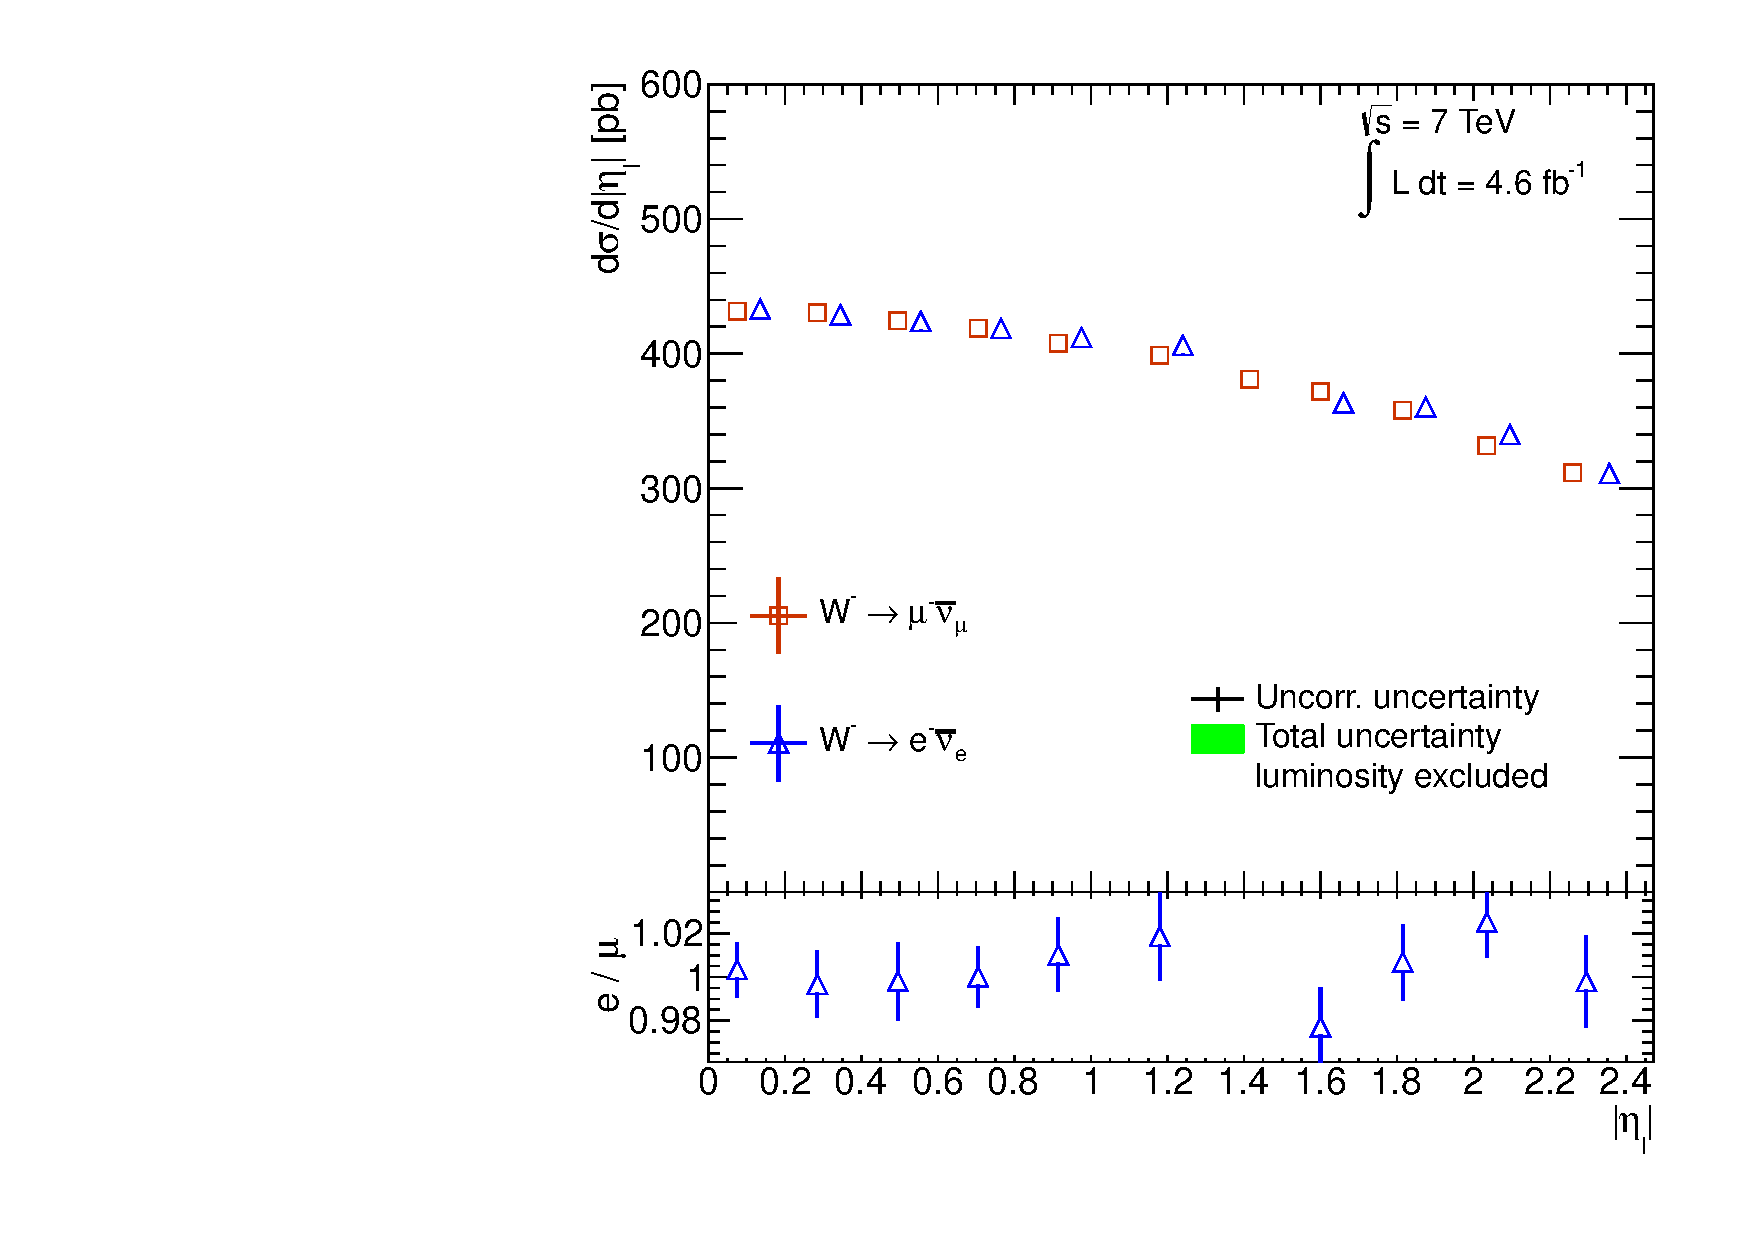
\includegraphics[width=1.0\textwidth]{dates/20130214/figures/plots/WMeta25_combined}

%% \cole
%% }

%% \slide{Single-differential Z}
%% {
%% \only<1>{ \small{ Z 46-66 GeV}}
%% \only<2>{ \small{ Z 66-116 GeV}}
%% \only<3>{ \small{ Z 116-150 GeV}}
%% \centering
%% \only<1> {
%% \includegraphics[width=0.7\textwidth]<1>{dates/20130214/figures/plots/Zlow_combined}
%% }
%% \only<2>{
%% \includegraphics[width=0.7\textwidth]<2>{dates/20130214/figures/plots/Zcen_combined}
%% }
%% \only<3>{
%% \includegraphics[width=0.7\textwidth]<3>{dates/20130214/figures/plots/Zhigh_combined}
%% }
%% }


%% \slide{Double-differential W}
%% {
%%   \only<1> {
%%     \begin{itemize}
%%     \item $W^+$
%%     \end{itemize}

%%   \begin{center}
%%     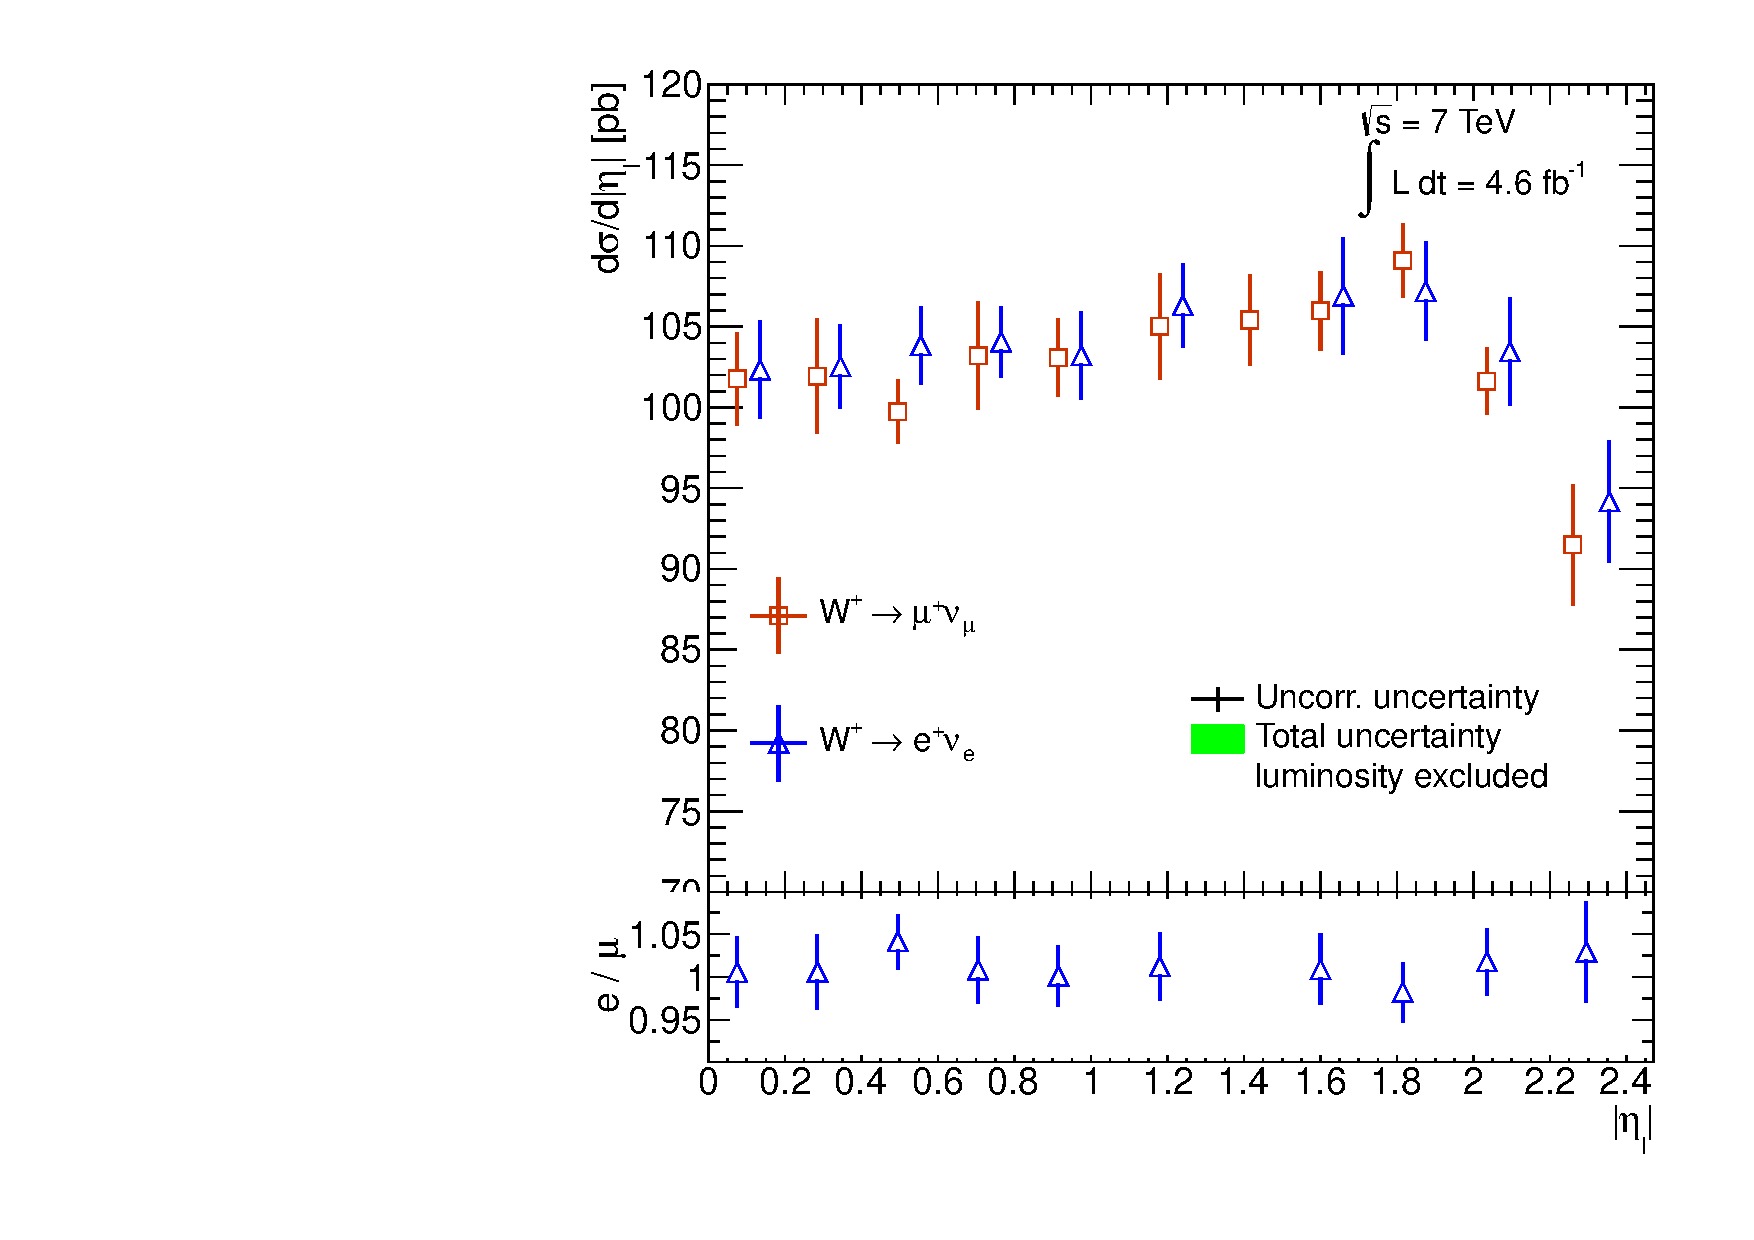
\includegraphics[width=0.3\textwidth]{dates/20130214/figures/plots/WPetaPt25-30_combined}
%%     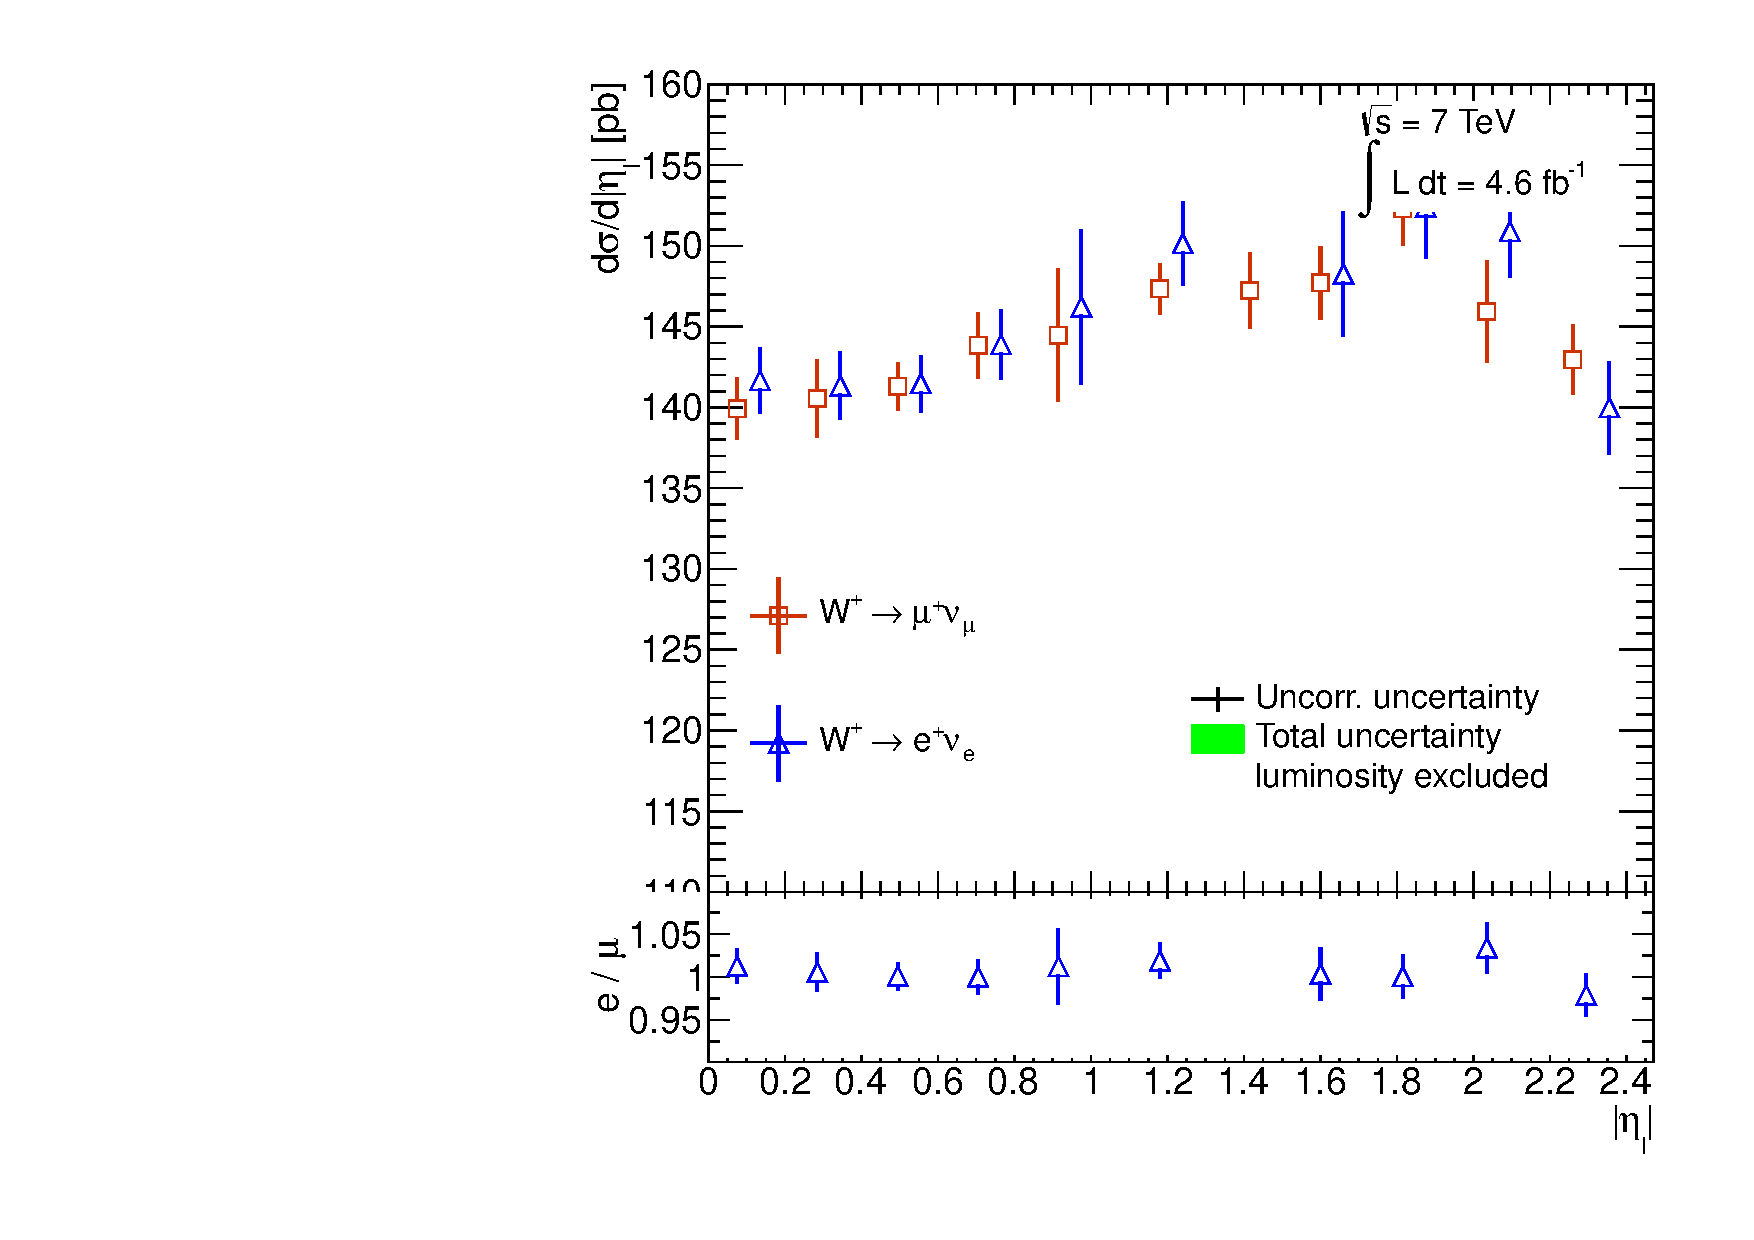
\includegraphics[width=0.3\textwidth]{dates/20130214/figures/plots/WPetaPt30-35_combined}
%%     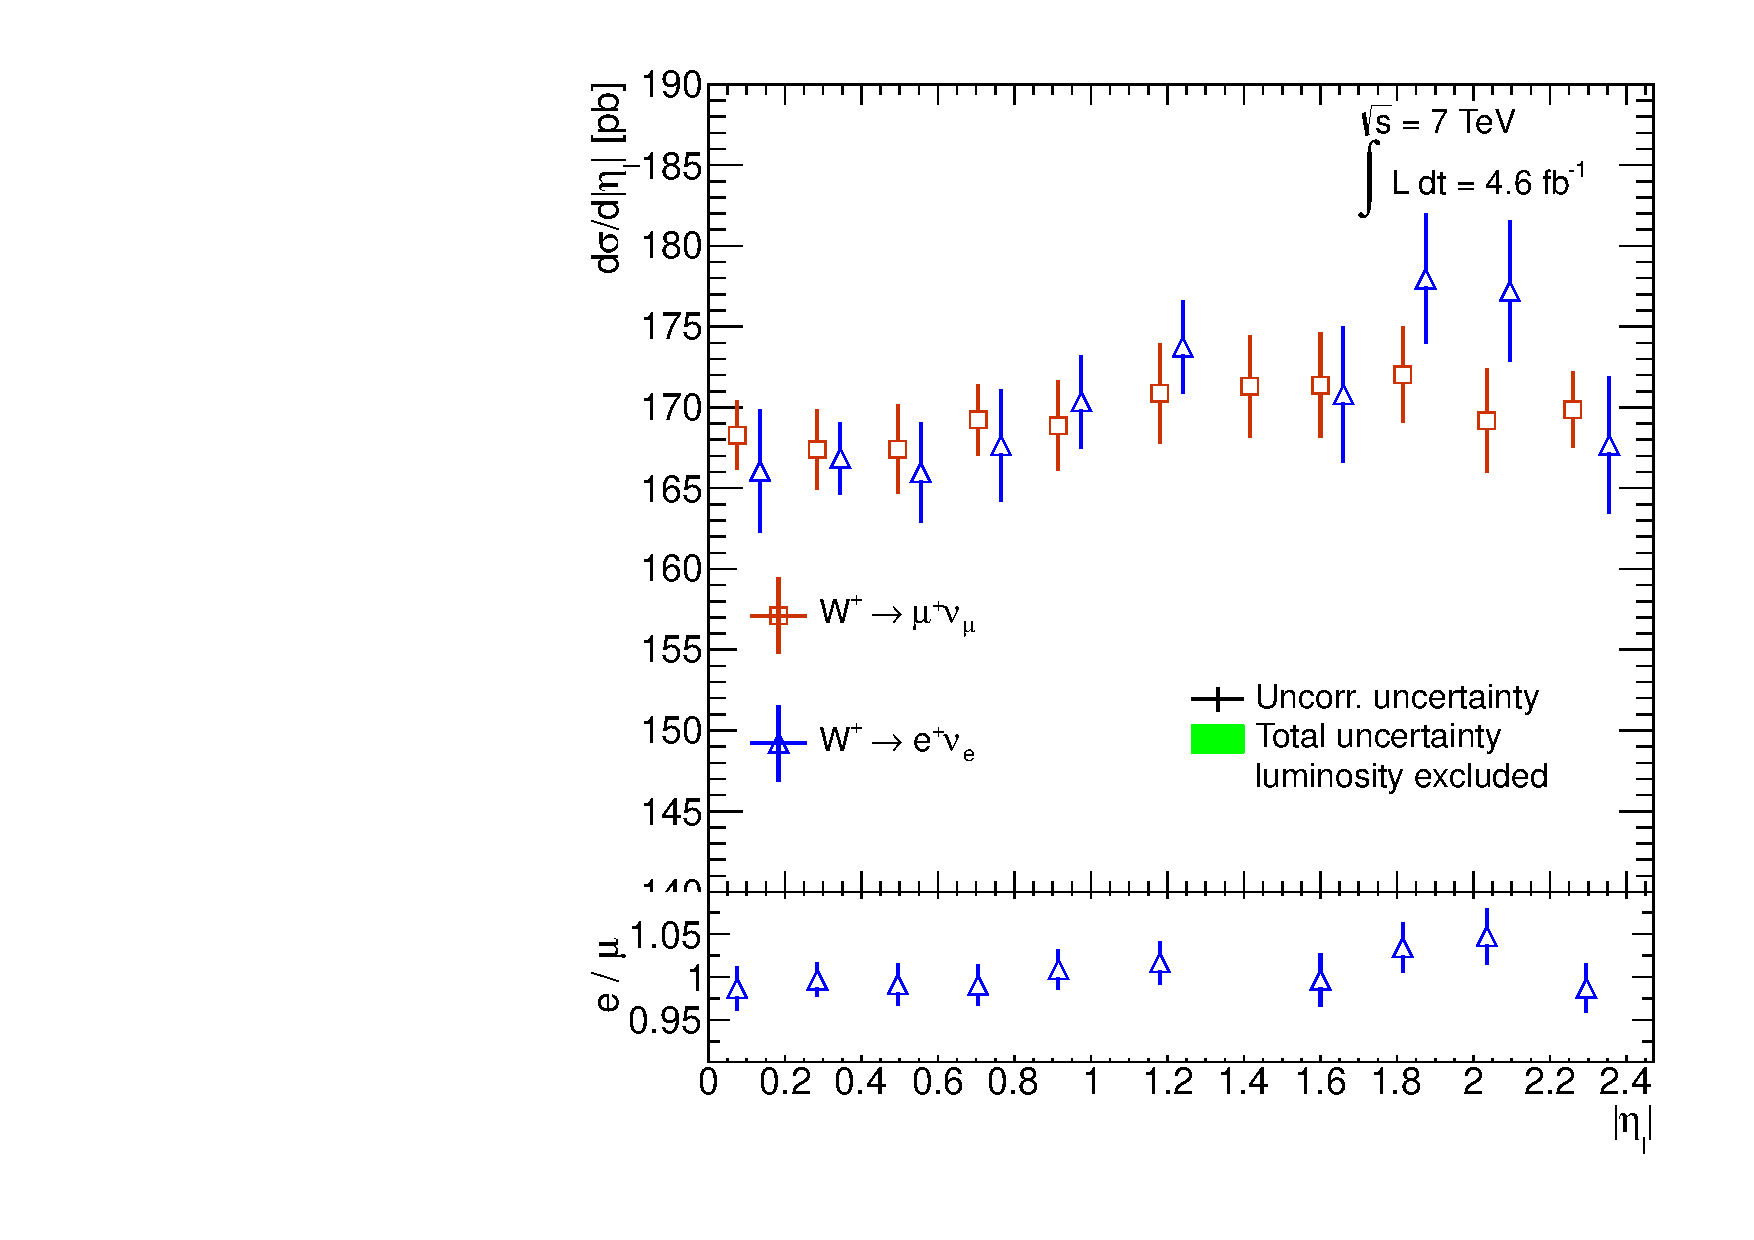
\includegraphics[width=0.3\textwidth]{dates/20130214/figures/plots/WPetaPt35-40_combined}
%%   \end{center}

%%   \begin{center}
%%     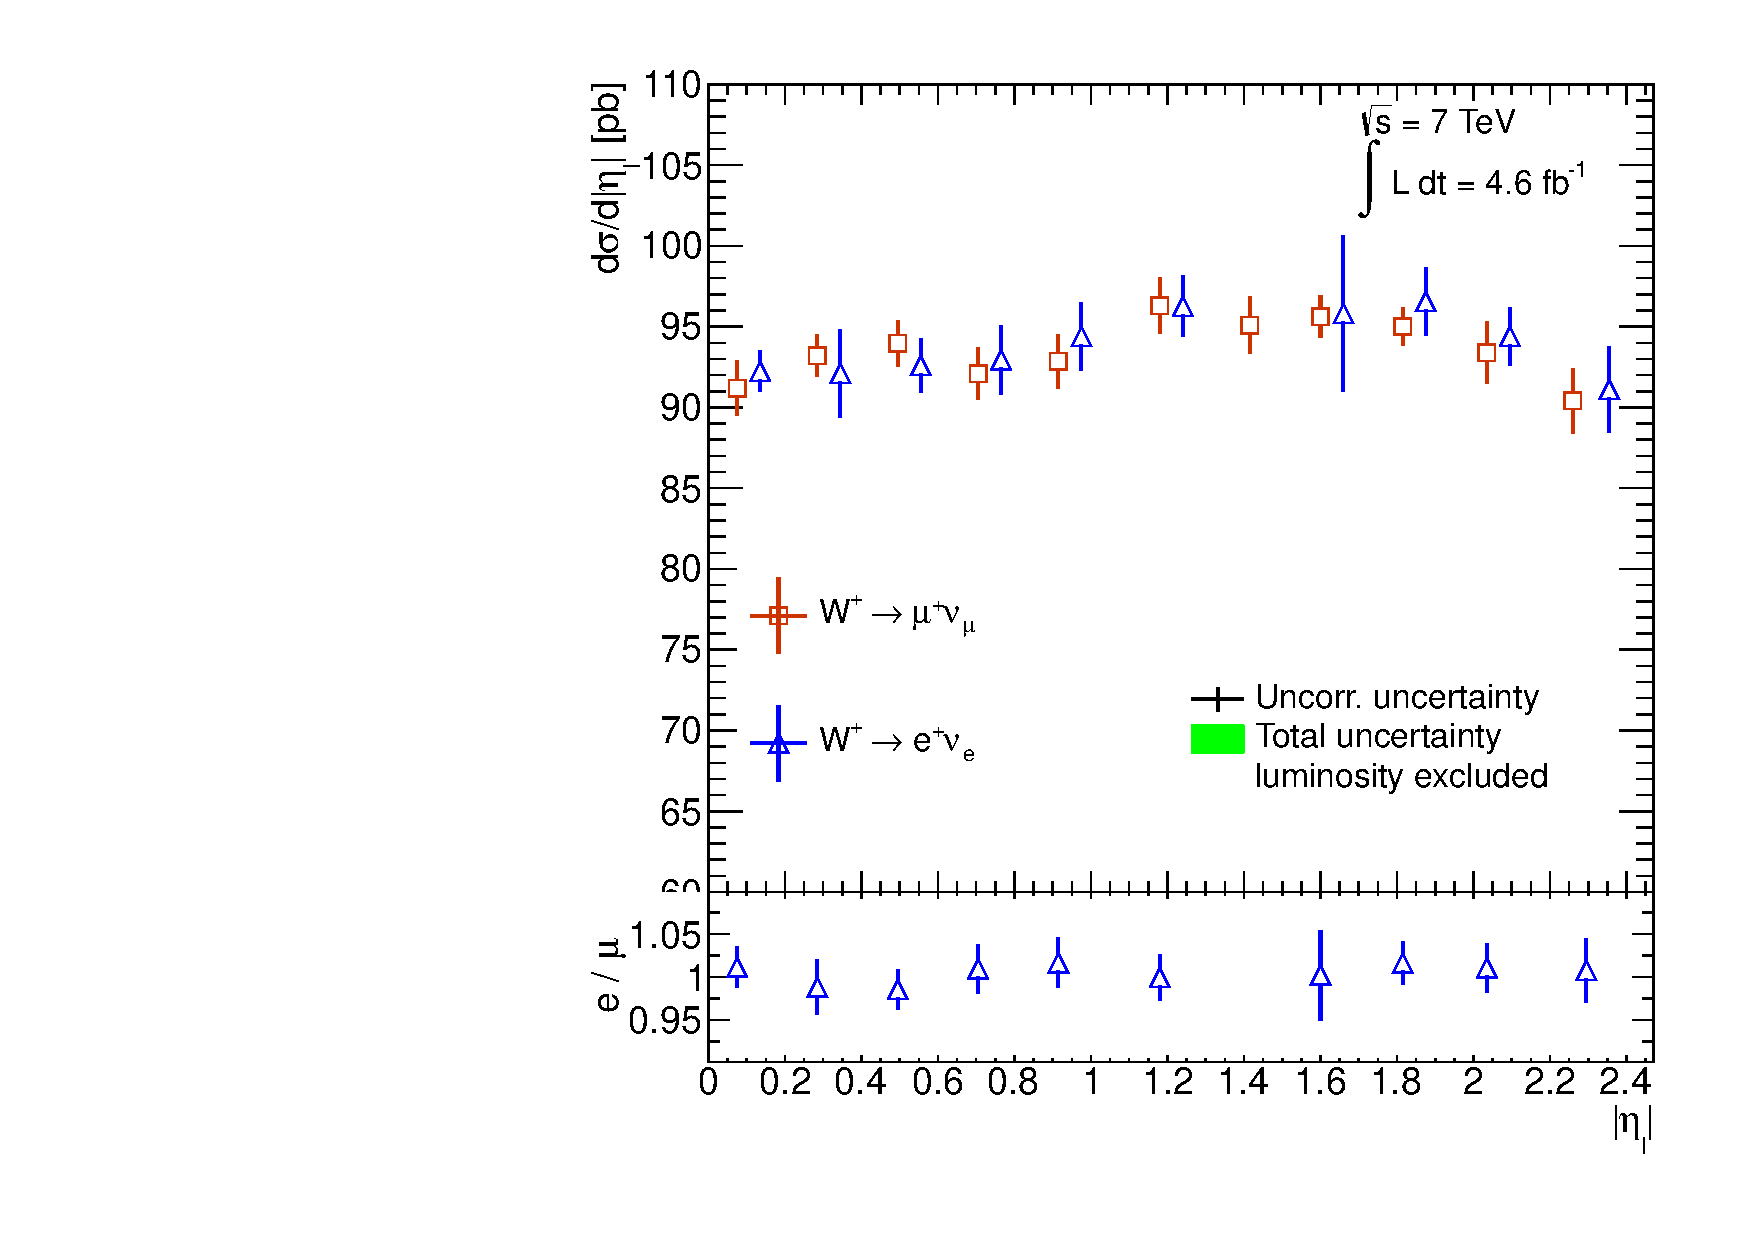
\includegraphics[width=0.3\textwidth]{dates/20130214/figures/plots/WPetaPt40-45_combined}
%%     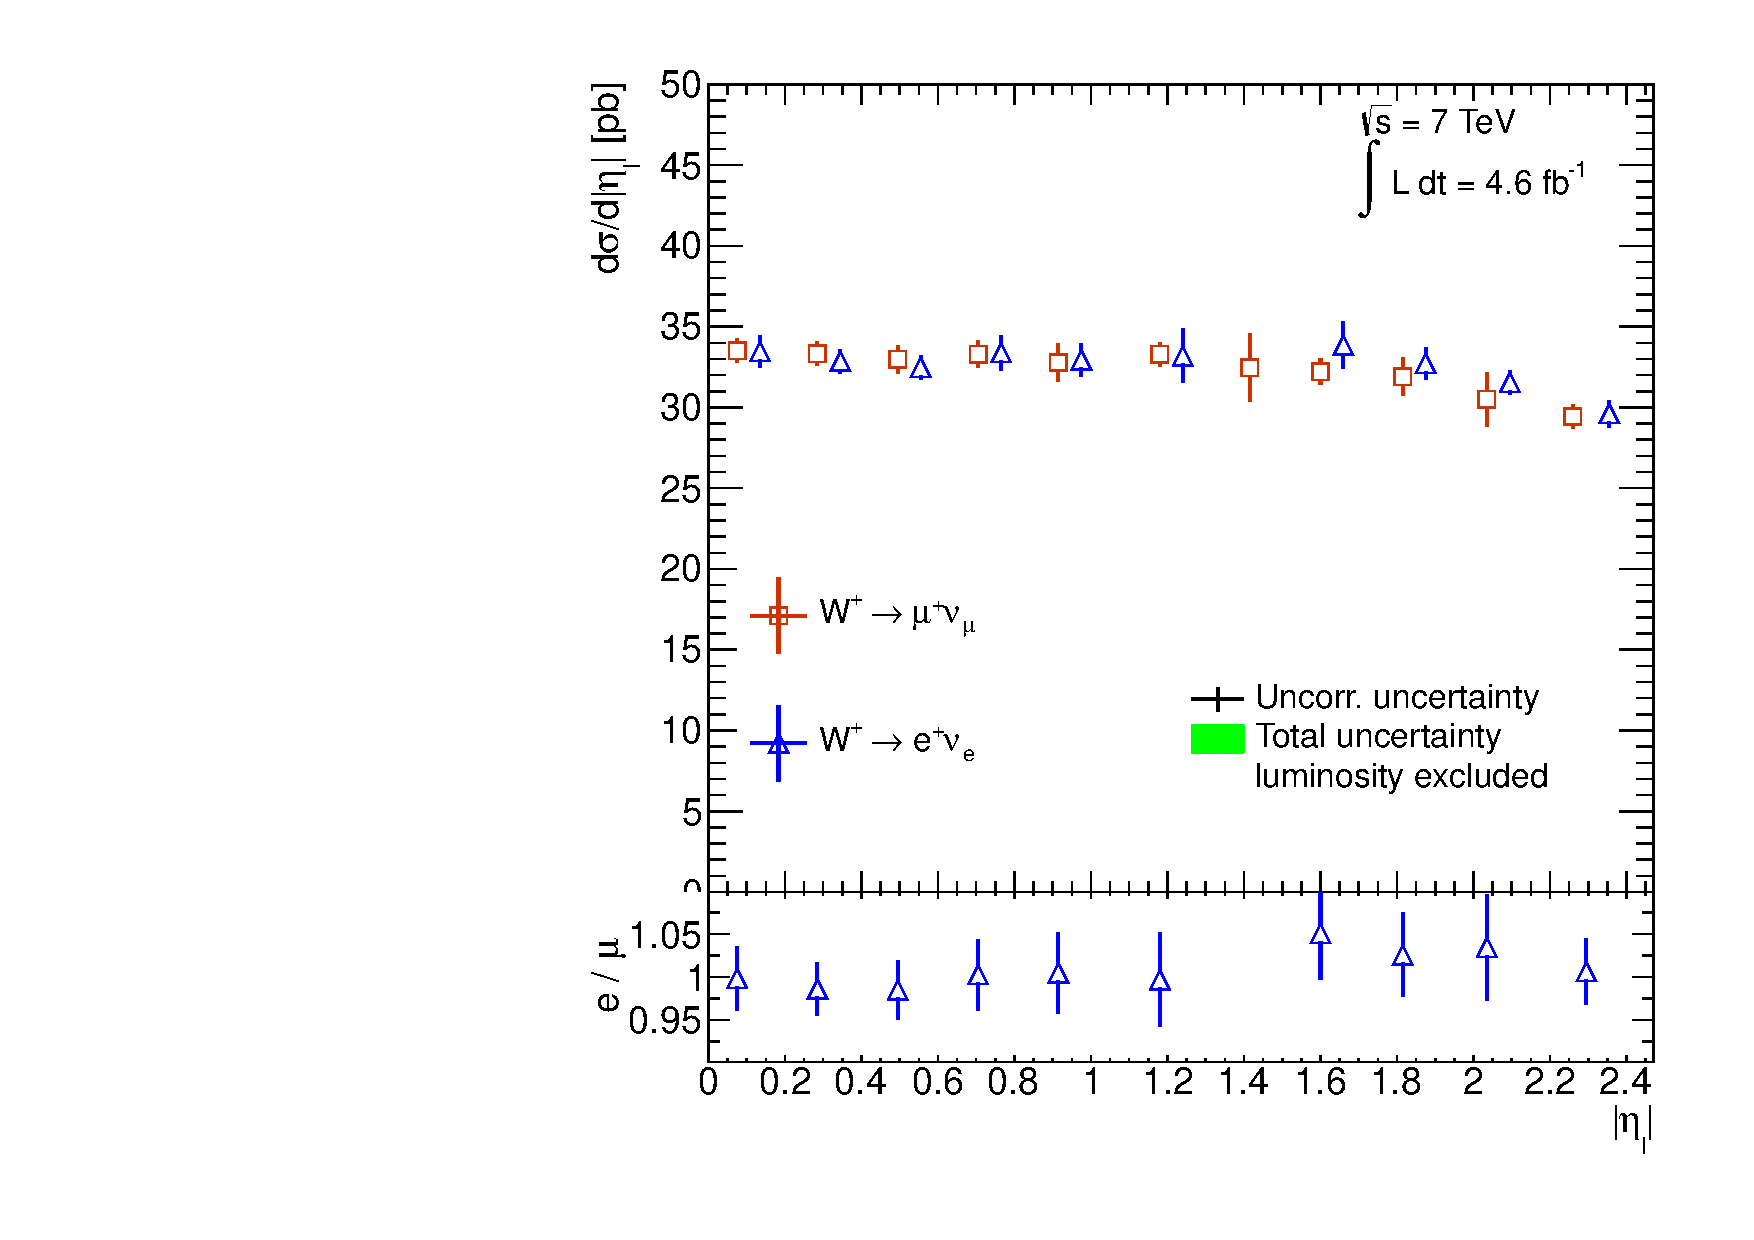
\includegraphics[width=0.3\textwidth]{dates/20130214/figures/plots/WPetaPt45-50_combined}
%%     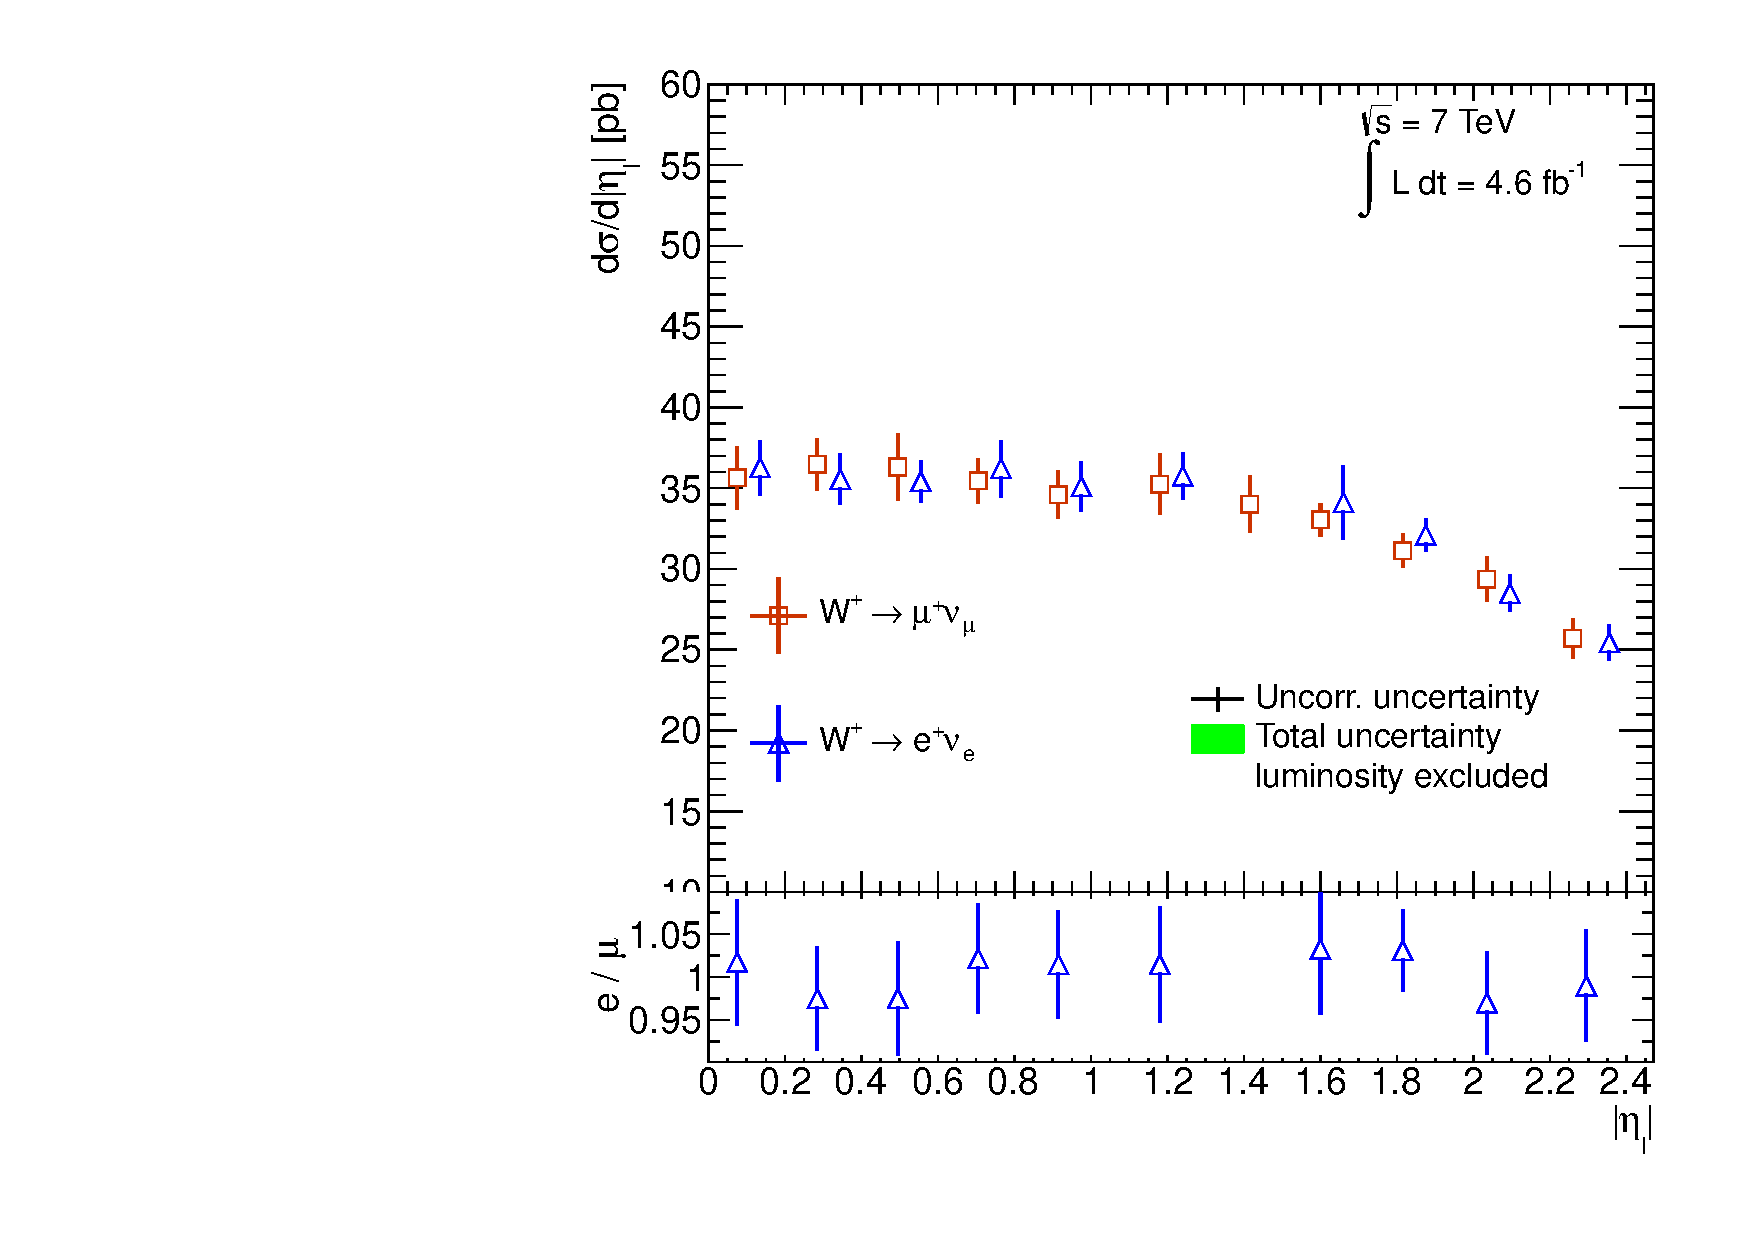
\includegraphics[width=0.3\textwidth]{dates/20130214/figures/plots/WPetaPt50_combined}
%%   \end{center}
%% }
%%   \only<2> {
%%     \begin{itemize}
%%     \item $W^-$
%%     \end{itemize}

%%   \begin{center}
%%     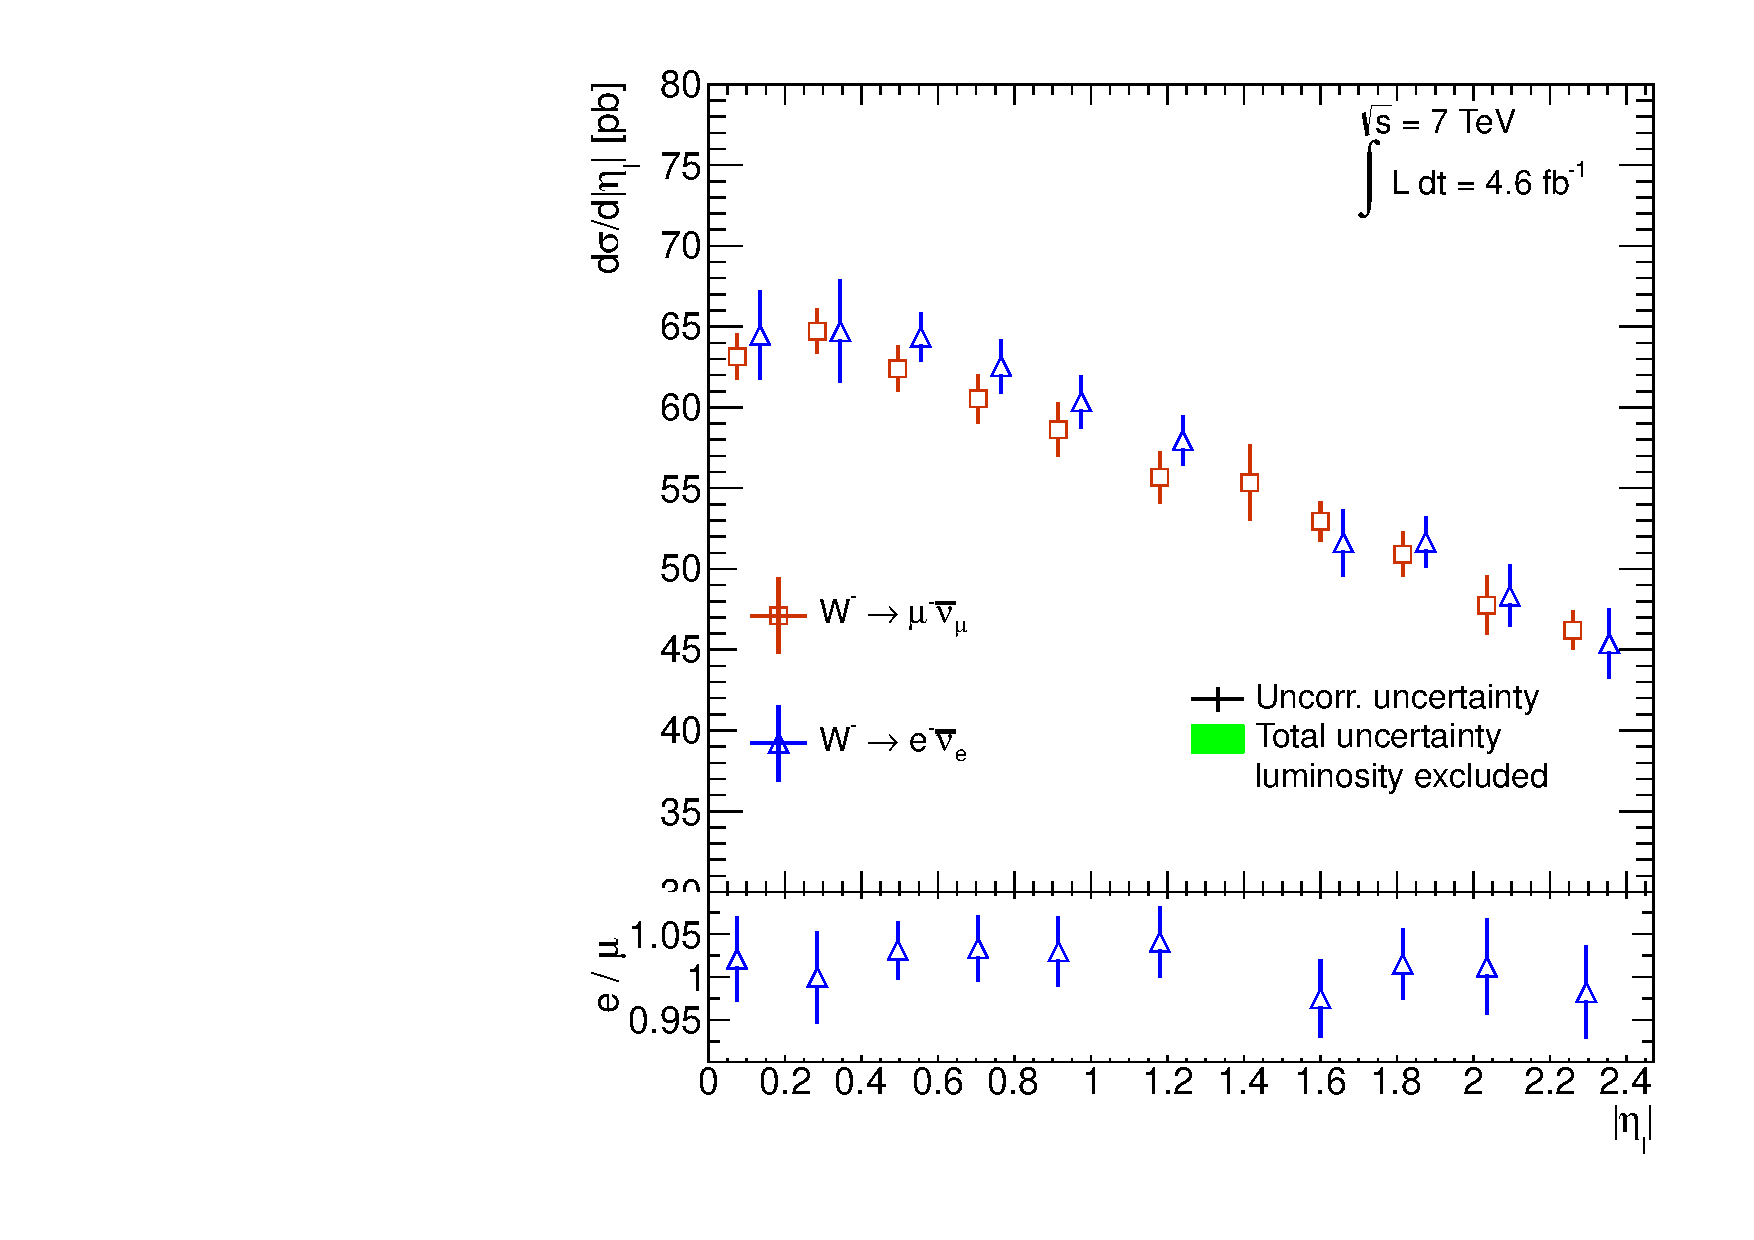
\includegraphics[width=0.3\textwidth]{dates/20130214/figures/plots/WMetaPt25-30_combined}
%%     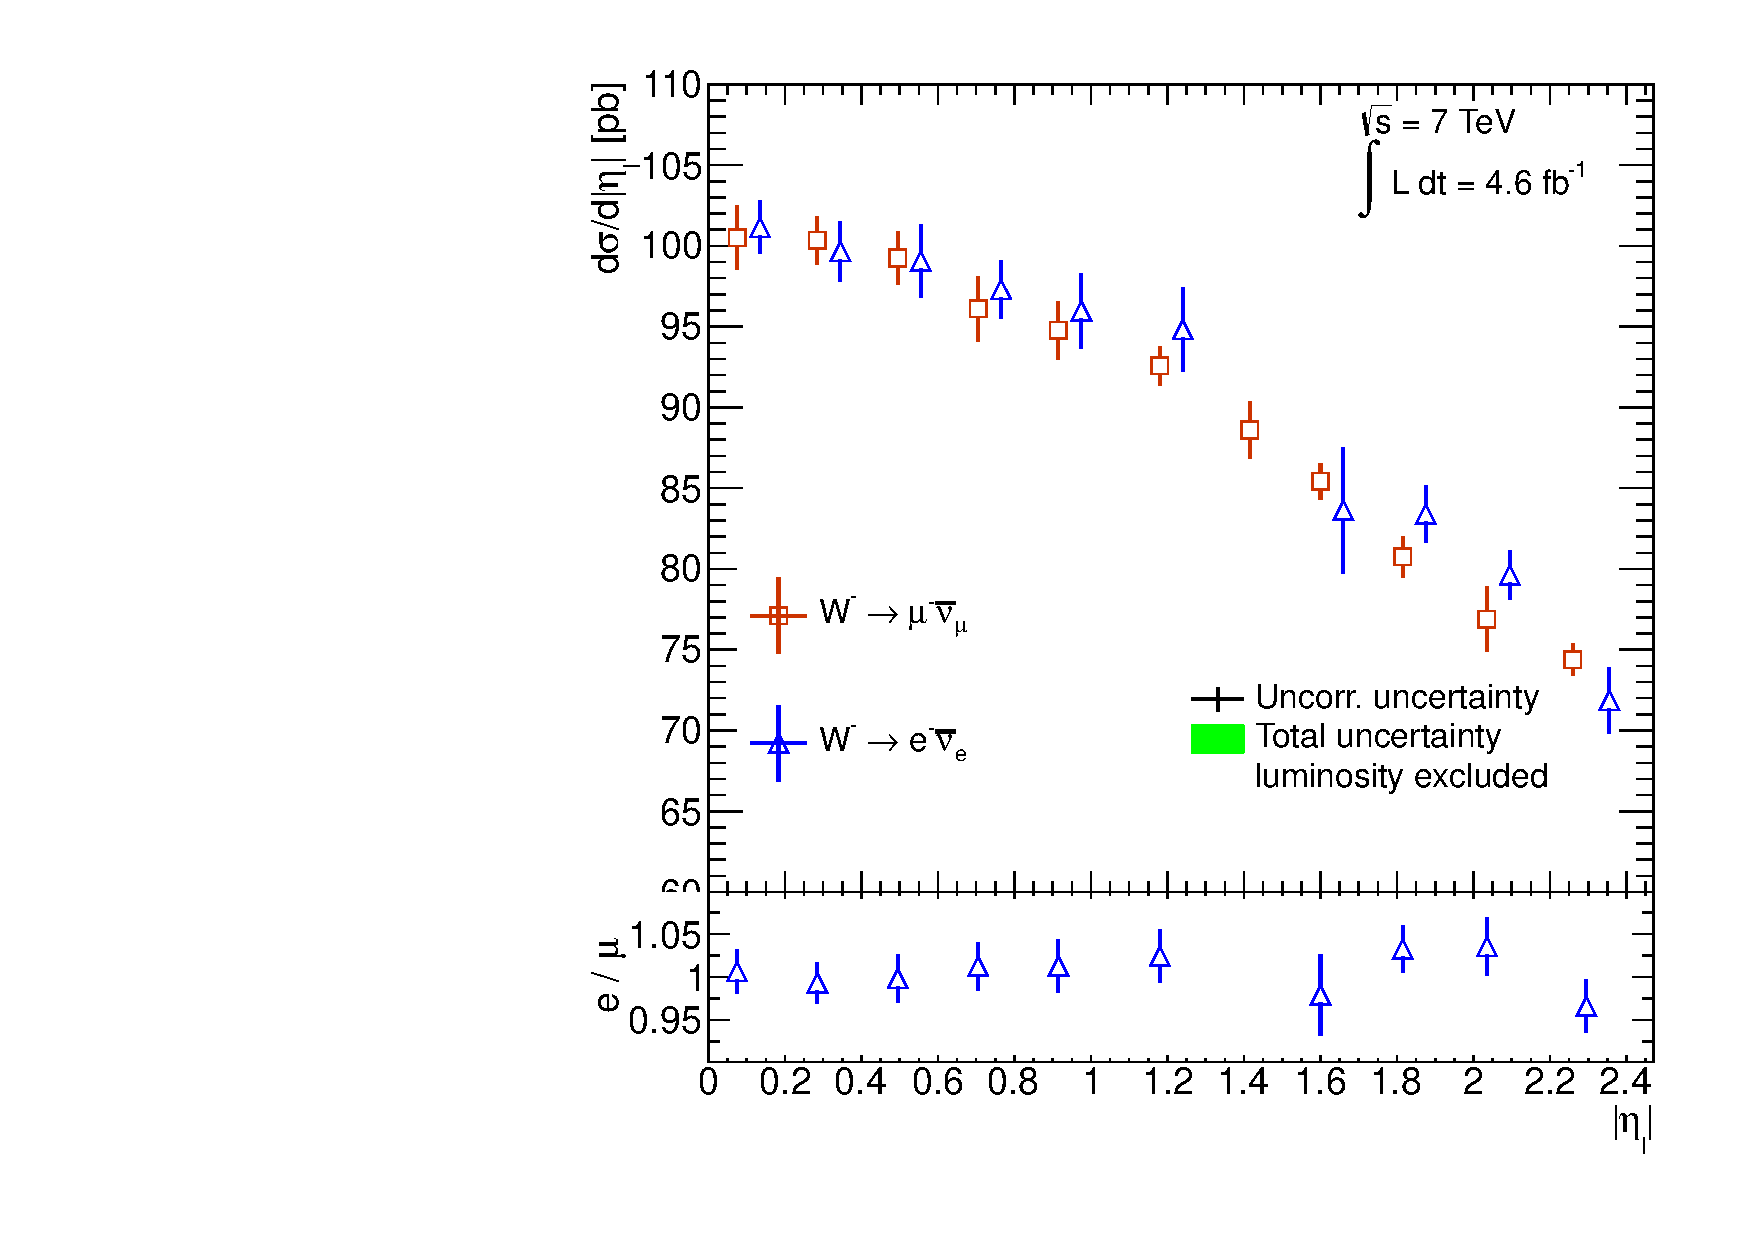
\includegraphics[width=0.3\textwidth]{dates/20130214/figures/plots/WMetaPt30-35_combined}
%%     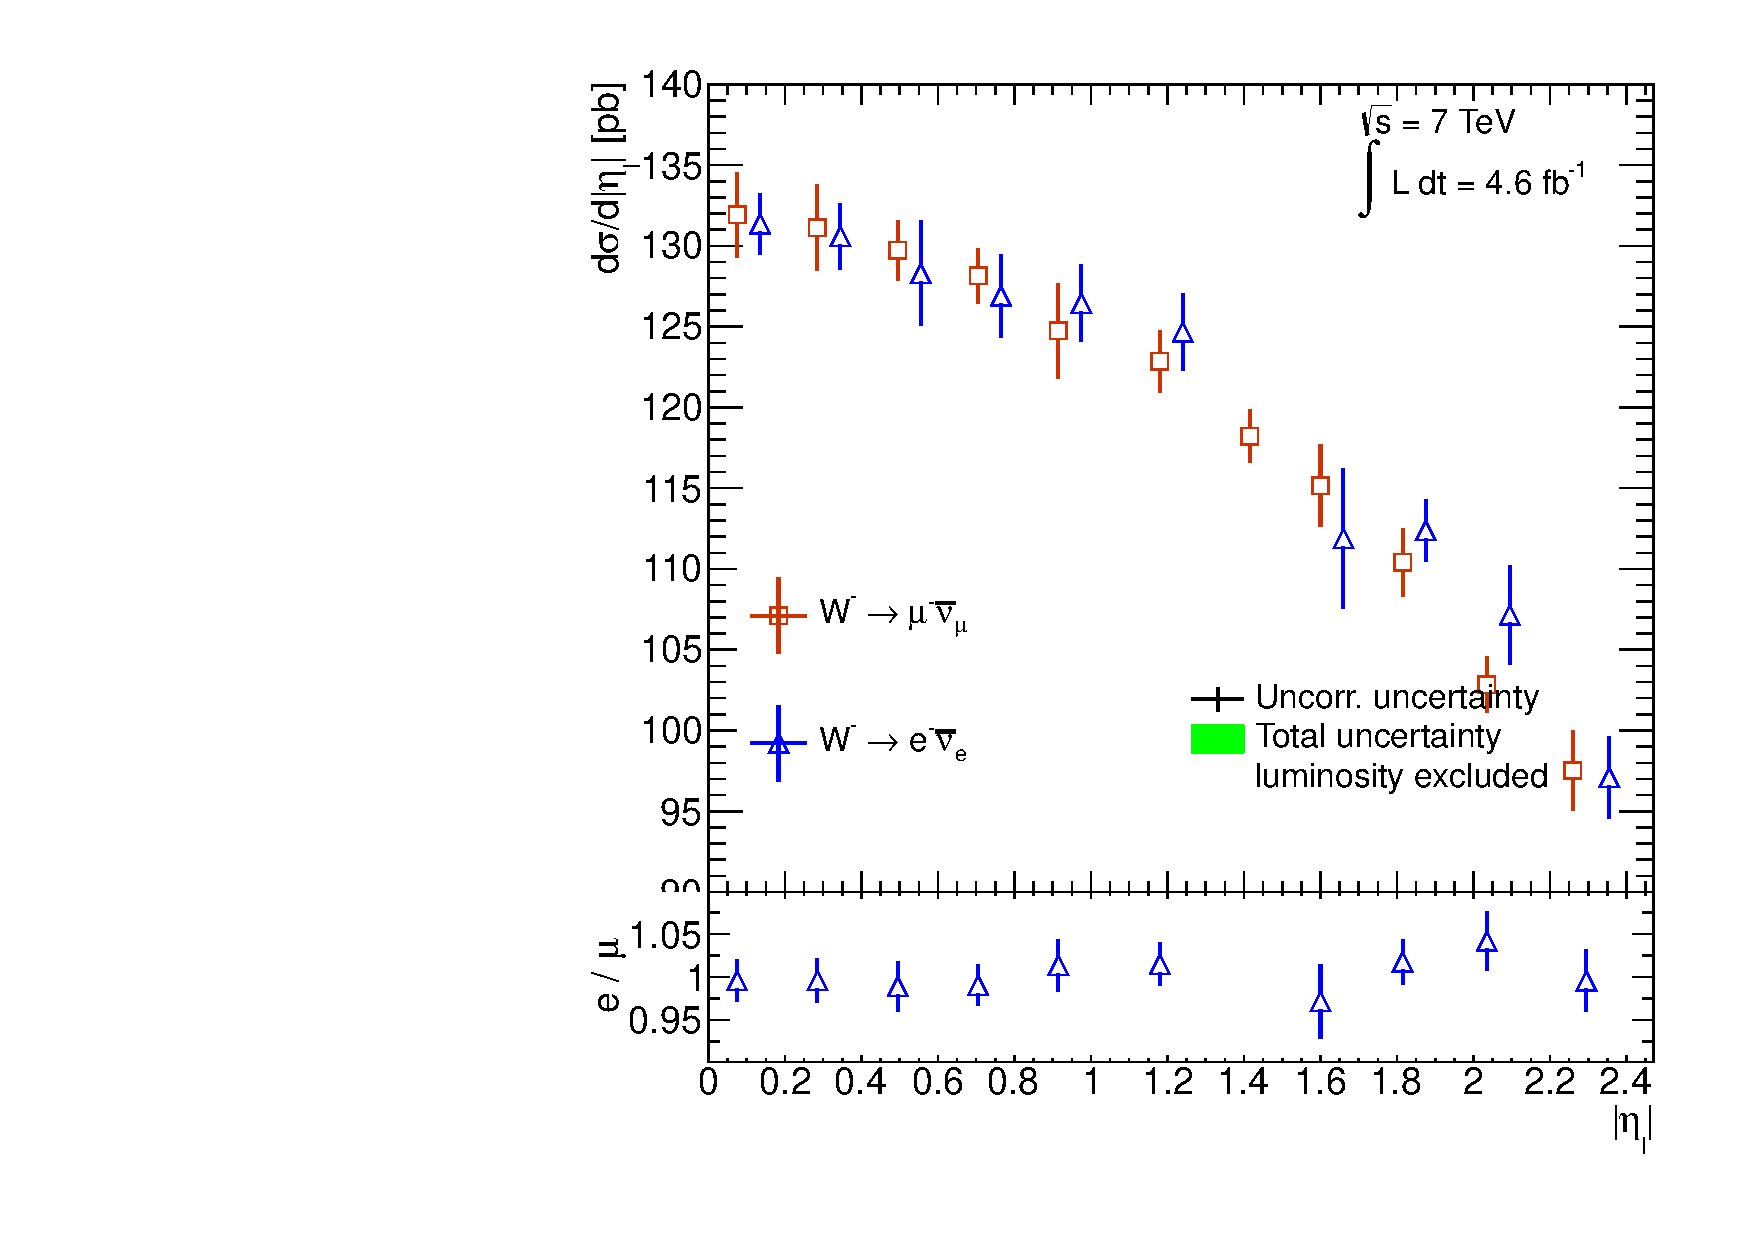
\includegraphics[width=0.3\textwidth]{dates/20130214/figures/plots/WMetaPt35-40_combined}
%%   \end{center}

%%   \begin{center}
%%     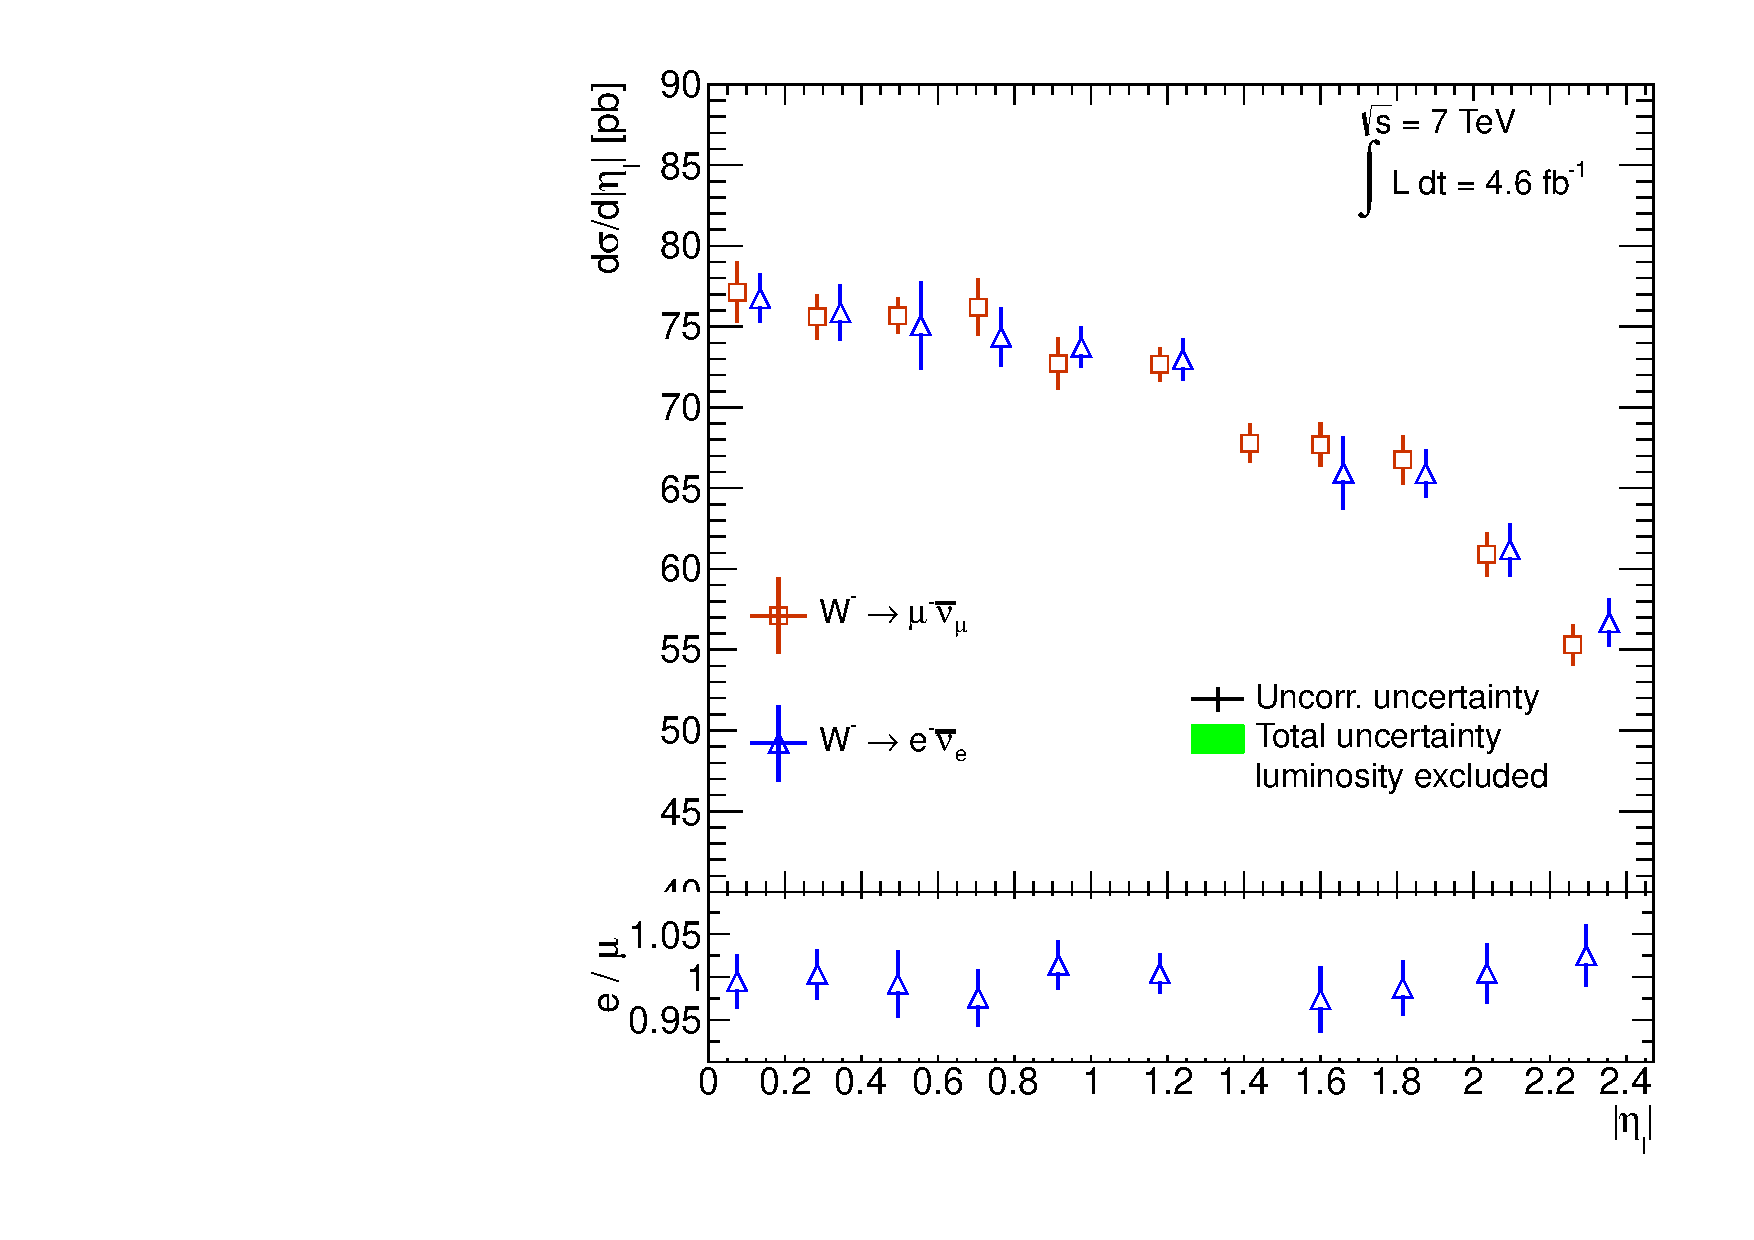
\includegraphics[width=0.3\textwidth]{dates/20130214/figures/plots/WMetaPt40-45_combined}
%%     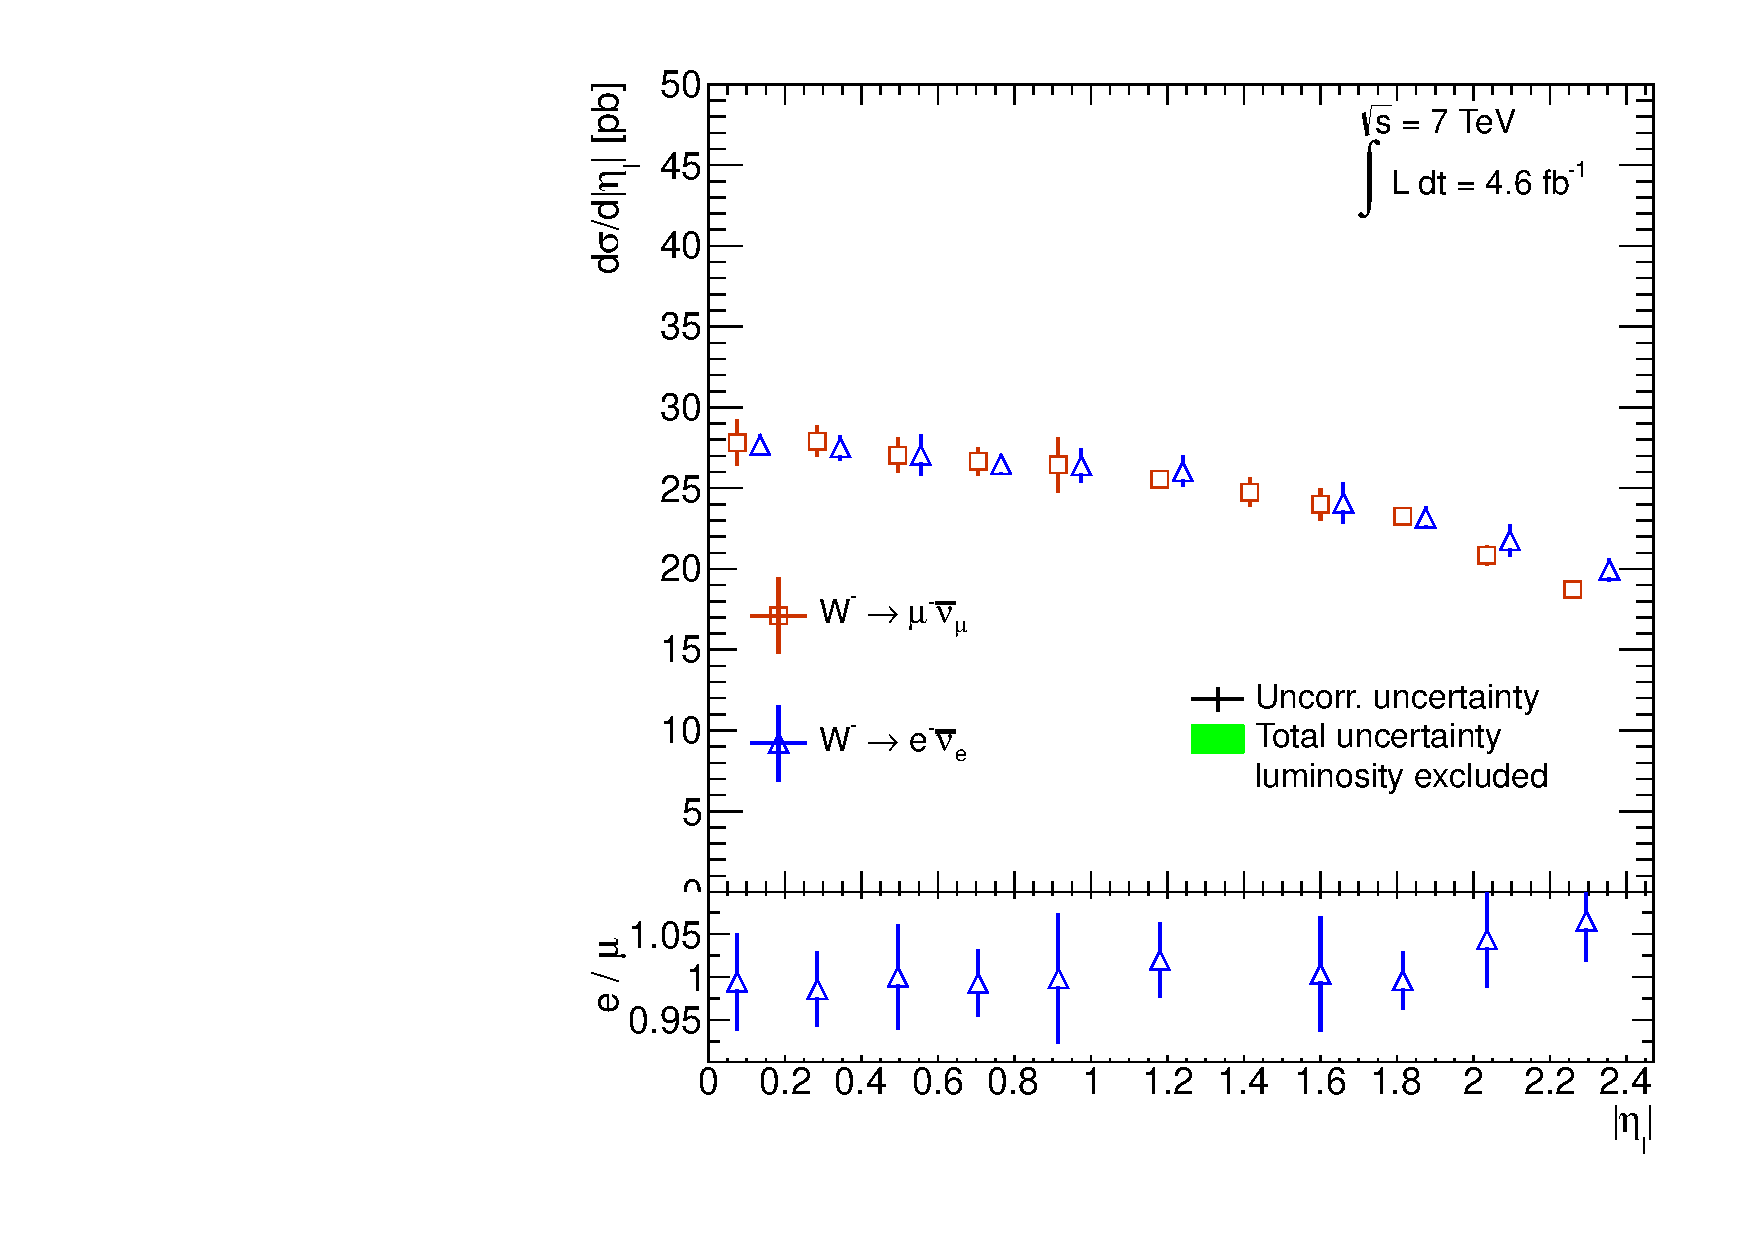
\includegraphics[width=0.3\textwidth]{dates/20130214/figures/plots/WMetaPt45-50_combined}
%%     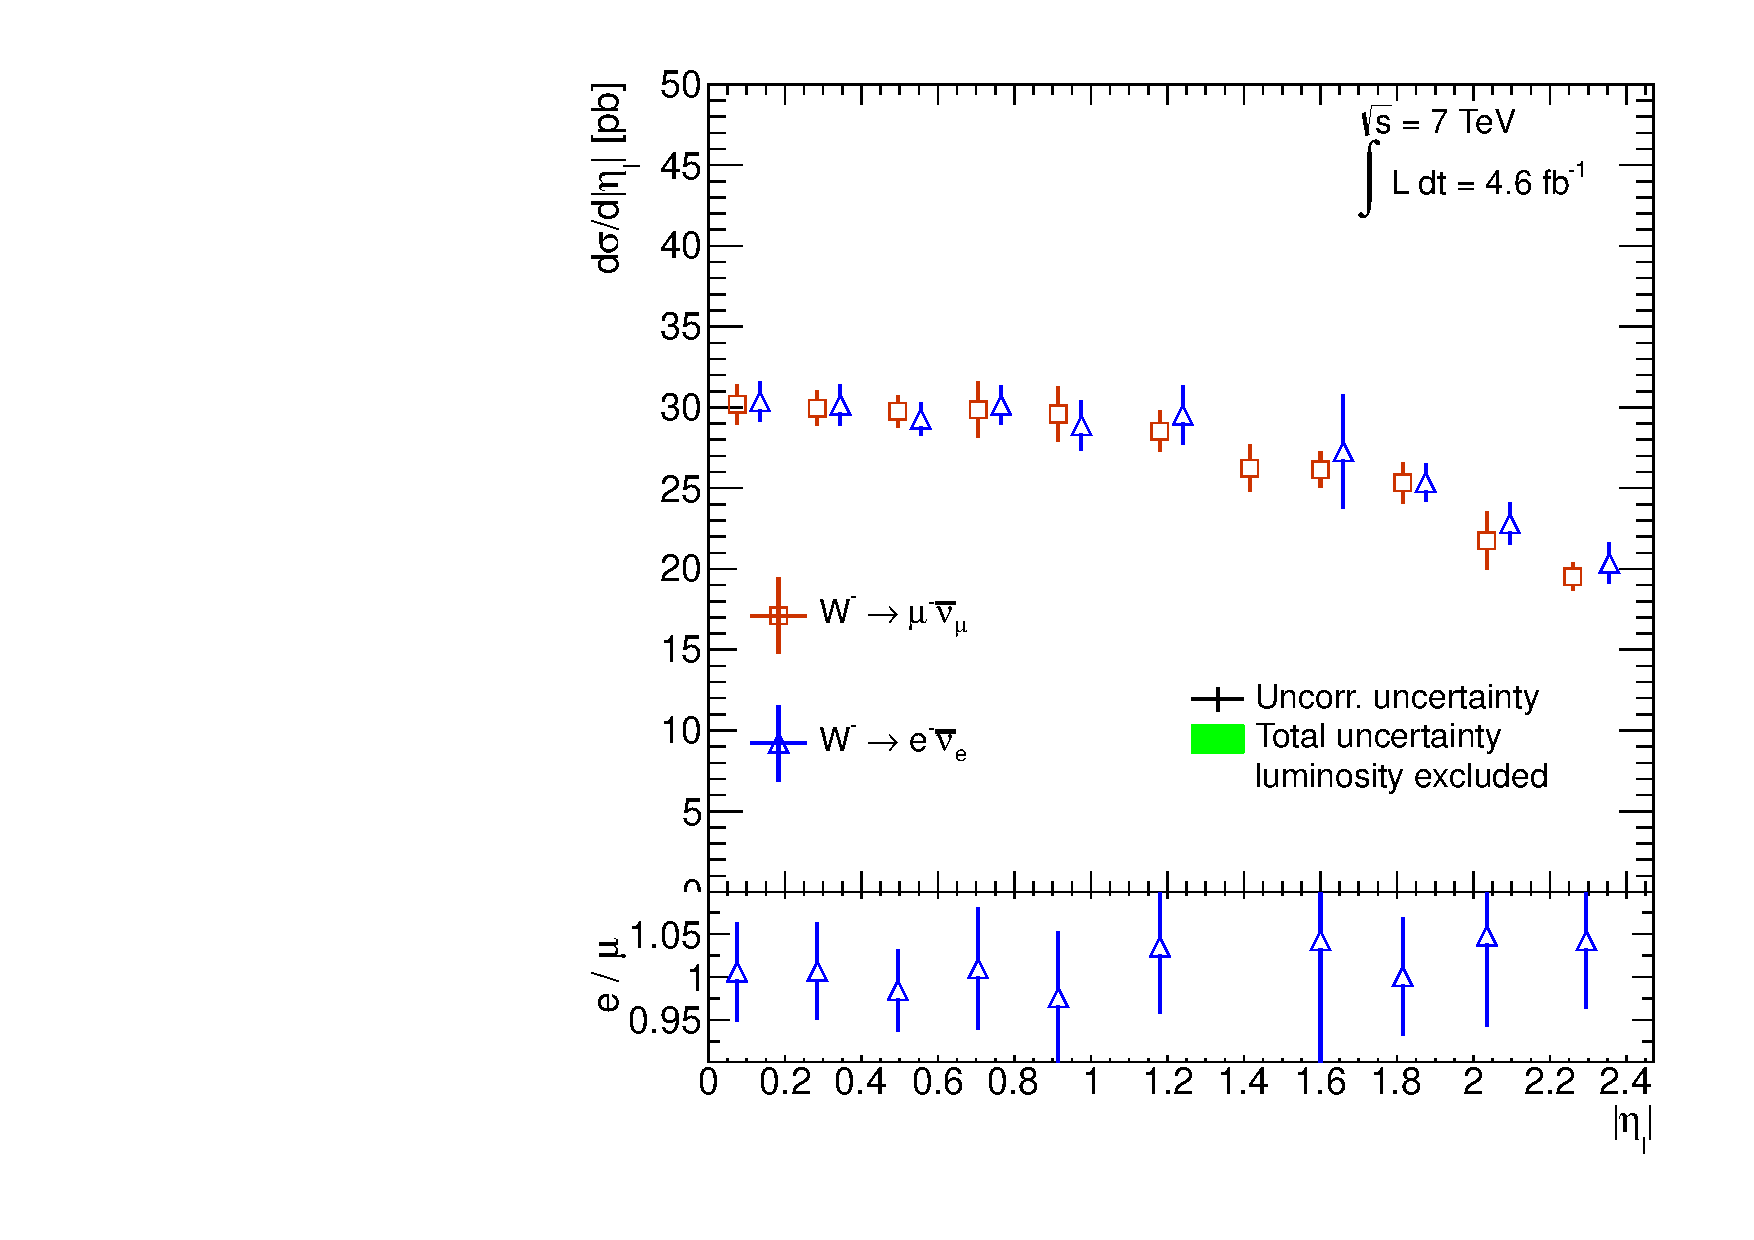
\includegraphics[width=0.3\textwidth]{dates/20130214/figures/plots/WMetaPt50_combined}
%%   \end{center}
%% }

%% }


%%
%% A/C side differences
%%
\slide{A-C side differences}
{
\centering
\Huge A-C side differences

}

\slide{ Final numbers: A/C for $W^-$ }
{
\small{
\begin{table}[tbph]
\centering
\begin{tabular}{lccccc}
\hline
\hline
$\eta$ bin & $XSEC_{|\eta|}^{ele}$ & $XSEC_{|\eta|}^{\mu}$ & $\delta$ & $XSEC_{Aside} - XSEC_{Cside}$ & $(A-C)/\delta$ \\
\hline

$0 < |\eta| <0.21$ & 433.0 & 431.5 & 4.0 & -9.4 & -2.3 \\
$0.21 < |\eta| <0.42$ & 428.9 & 430.3 & 4.1 & -2.1 & -0.5 \\
$0.42 < |\eta| <0.63$ & 423.8 & 424.6 & 4.7 & -6.8 & -1.5 \\
$0.63 < |\eta| <0.84$ & 418.8 & 418.7 & 3.7 & 6.8 & 1.8 \\
$0.84 < |\eta| <1.05$ & 412.0 & 407.8 & 5.1 & 11.5 & 2.3 \\
$1.05 < |\eta| <1.37$ & 406.2 & 398.8 & 5.1 & 1.4 & 0.3 \\
$1.37 < |\eta| <1.52$ & 199.1 & 380.9 & 4.5 & 1.3 & 0.3 \\
$1.52 < |\eta| <1.74$ & 199.1 & 371.9 & 4.1 & 4.9 & 1.2 \\
$1.74 < |\eta| <1.95$ & 360.4 & 358.0 & 5.1 & 4.3 & 0.9 \\
$1.95 < |\eta| <2.18$ & 339.9 & 331.5 & 3.9 & 19.4 & \color{red}{5.0} \\
$2.18 < |\eta| <2.4$ & 312.4 & 316.4 & 3.6 & -0.5 & -0.1 \\

\hline
\end{tabular}
\caption{Studying A-side vs C-side differences for $W^{-} \rightarrow \mu^{-} \nu$.}
\label{tab:NEG}
\end{table}
}
}

\slide{ Final numbers: A/C for $W^+$ }
{
\small{
\begin{table}[tbph]
\centering
\begin{tabular}{lccccc}
\hline
\hline
$\eta$ bin & $XSEC_{|\eta|}^{ele}$ & $XSEC_{|\eta|}^{\mu}$ & $\delta$ & $XSEC_{Aside} - XSEC_{Cside}$ & $(A-C)/\delta$ \\
\hline

$0 < |\eta| <0.21$ & 572.5 & 570.5 & 4.6 & 1.9 & 0.4 \\
$0.21 < |\eta| <0.42$ & 571.4 & 573.9 & 4.6 & -1.7 & -0.4 \\
$0.42 < |\eta| <0.63$ & 572.5 & 572.9 & 6.9 & 0.8 & 0.1 \\
$0.63 < |\eta| <0.84$ & 579.0 & 578.0 & 4.5 & 14.3 & \color{red}{3.2} \\
$0.84 < |\eta| <1.05$ & 582.6 & 577.9 & 5.2 & 7.1 & 1.4 \\
$1.05 < |\eta| <1.37$ & 596.2 & 589.2 & 5.7 & 8.9 & 1.6 \\
$1.37 < |\eta| <1.52$ & 320.0 & 586.2 & 6.2 & 7.3 & 1.2 \\
$1.52 < |\eta| <1.74$ & 320.0 & 586.9 & 5.4 & 26.5 & \color{red}{4.9} \\
$1.74 < |\eta| <1.95$ & 596.9 & 591.2 & 4.2 & 13.3 & \color{red}{3.1} \\
$1.95 < |\eta| <2.18$ & 584.8 & 570.7 & 7.0 & 32.4 & \color{red}{4.6} \\
$2.18 < |\eta| <2.4$ & 549.4 & 558.3 & 6.4 & 10.2 & 1.6 \\

\hline
\end{tabular}
\caption{Studying A-side vs C-side differences for $W^{+} \rightarrow \mu^{+} \nu$.}
\label{tab:POS}
\end{table}
}
}

\slide{ A-C ratios: data-driven vs MC QCD }
{

\only<1>{
 A/C ratios for data, background-subtracted data, and signal MC. \\
 The shaded errors on the ratio (in the following plots) are correct. \\
 Here, we are considering the \red{effects of QCD subtraction}. \\
 \small{(for all subsequent studies, MC-based QCD will be used for simplicity)}
}
\only<4>{
  Conclusion: on the scale of existing disagreements, the choice of QCD templates has a minor effect.
}

\colb[T]

\column{.5\textwidth}
\centering
\only<2>{ \small{ Data-driven QCD: $W^{+}$}}
\only<3>{ \small{ Heavy-flavor MC QCD: $W^{+}$}}
\includegraphics[width=1.0\textwidth]<2>{dates/20130214/figures/AC/W_NOM_Q4_stack_d3_eta_lpt_met_y_2__1_z_0__1_POS}
\includegraphics[width=1.0\textwidth]<3>{dates/20130214/figures/AC/W_NOM_Q0_stack_d3_eta_lpt_met_y_2__1_z_0__1_POS}

\column{.5\textwidth}
\centering
\only<2>{ \small{ Data-driven QCD: $W^{-}$}}
\only<3>{ \small{ Heavy-flavor MC QCD: $W^{-}$}}
\includegraphics[width=1.0\textwidth]<2>{dates/20130214/figures/AC/W_NOM_Q4_stack_d3_eta_lpt_met_y_2__1_z_0__1_NEG}
\includegraphics[width=1.0\textwidth]<3>{dates/20130214/figures/AC/W_NOM_Q0_stack_d3_eta_lpt_met_y_2__1_z_0__1_NEG}

\cole
}


\slide{ A-C ratios: playing with reco/trigger scale factors }
{

\only<1>{
 A/C ratios for data, background-subtracted data, and signal MC. \\
 The shaded errors on the ratio (in the following plots) are correct. \\
 Here, we are considering the \red{effects of reco/trigger scale factors}. \\
 \small{(sorry, no systematic bands in the following set of plots)}
}
\only<6>{
  Conclusion: trigger scale factors have a major effect, especially in the barrel. \\
  However, they don't seen to provide a substantial A/C correction in the endcaps.
}


\colb[T]

\column{.5\textwidth}
\centering
\only<2>{ \small{ Nominal: $W^{+}$}}
\only<3>{ \small{ Without reco SF: $W^{+}$}}
\only<4>{ \small{ Without trigger SF: $W^{+}$}}
\only<5>{ \small{ Without either SF: $W^{+}$}}
\includegraphics[width=1.0\textwidth]<2>{dates/20130214/figures/AC/WNT_NOM_Q0_stack_lepton_etav_POS}
\includegraphics[width=1.0\textwidth]<3>{dates/20130214/figures/AC/WNT_NORECSF_Q0_stack_lepton_etav_POS}
\includegraphics[width=1.0\textwidth]<4>{dates/20130214/figures/AC/WNT_NOTRIGSF_Q0_stack_lepton_etav_POS}
\includegraphics[width=1.0\textwidth]<5>{dates/20130214/figures/AC/WNT_NOSF_Q0_stack_lepton_etav_POS}

\column{.5\textwidth}
\centering
\only<2>{ \small{ Nominal: $W^{-}$}}
\only<3>{ \small{ Without reco SF: $W^{-}$}}
\only<4>{ \small{ Without trigger SF: $W^{-}$}}
\only<5>{ \small{ Without either SF: $W^{-}$}}
\includegraphics[width=1.0\textwidth]<2>{dates/20130214/figures/AC/WNT_NOM_Q0_stack_lepton_etav_NEG}
\includegraphics[width=1.0\textwidth]<3>{dates/20130214/figures/AC/WNT_NORECSF_Q0_stack_lepton_etav_NEG}
\includegraphics[width=1.0\textwidth]<4>{dates/20130214/figures/AC/WNT_NOTRIGSF_Q0_stack_lepton_etav_NEG}
\includegraphics[width=1.0\textwidth]<5>{dates/20130214/figures/AC/WNT_NOSF_Q0_stack_lepton_etav_NEG}

\cole
}


\slide{ A-C ratios: playing with kinematic regions }
{

\only<1>{
 A/C ratios for data, background-subtracted data, and signal MC. \\
 The shaded errors on the ratio (in the following plots) are correct. \\
 Here, we are considering the \red{effects of different kinematic cuts}. \\
 \small{(sorry, no systematic bands in the following set of plots)}
}
\only<5>{
  Conclusion: disagreements persist even in higher-pT kinematic regions.
}

\colb[T]

\column{.5\textwidth}
\centering
\only<2>{ \small{ Nominal: $p_T>20, met>25, wmt>40$, $W^{+}$}}
\only<3>{ \small{ Nominal: $p_T>25, met>25, wmt>40$, $W^{+}$}}
\only<4>{ \small{ Nominal: $p_T>20, met>35, wmt>50$, $W^{+}$}}
\includegraphics[width=1.0\textwidth]<2>{dates/20130214/figures/AC/WNT_NOM_Q0_stack_lepton_etav_POS}
\includegraphics[width=1.0\textwidth]<3>{dates/20130214/figures/AC/WNT_PT25_Q0_stack_lepton_etav_POS}
\includegraphics[width=1.0\textwidth]<4>{dates/20130214/figures/AC/WNT_MET35WMT50_Q0_stack_lepton_etav_POS}

\column{.5\textwidth}
\centering
\only<2>{ \small{ Nominal: $p_T>20, met>25, wmt>40$, $W^{-}$}}
\only<3>{ \small{ Nominal: $p_T>25, met>25, wmt>40$, $W^{-}$}}
\only<4>{ \small{ Nominal: $p_T>20, met>35, wmt>50$, $W^{-}$}}
\includegraphics[width=1.0\textwidth]<2>{dates/20130214/figures/AC/WNT_NOM_Q0_stack_lepton_etav_NEG}
\includegraphics[width=1.0\textwidth]<3>{dates/20130214/figures/AC/WNT_PT25_Q0_stack_lepton_etav_NEG}
\includegraphics[width=1.0\textwidth]<4>{dates/20130214/figures/AC/WNT_MET35WMT50_Q0_stack_lepton_etav_NEG}

\cole
}


\slide{ A-C ratios: choice of MET }
{

\only<1>{
 A/C ratios for data, background-subtracted data, and signal MC. \\
 The shaded errors on the ratio (in the following plots) are correct. \\
 Here, we are considering the \red{effects of a different MET: corrected LocHadTopo}. \\
 \small{(the same MET that was used in the 2010 measurement)} \\
 \small{(sorry, no systematic bands in the following set of plots)}
}

\only<4>{
  Conclusion: disagreements persist even with LocHadTopo, although overall things move around a bit.
}

\colb[T]

\column{.5\textwidth}
\centering
\only<2>{ \small{ Nominal: MetRefFinal, $W^{+}$}}
\only<3>{ \small{ Nominal: LocHadTopo(corr), $W^{+}$}}
\includegraphics[width=1.0\textwidth]<2>{dates/20130214/figures/AC/WNT_NOM_Q0_stack_lepton_etav_POS}
\includegraphics[width=1.0\textwidth]<3>{dates/20130214/figures/AC/WNT_METLH_Q0_stack_lepton_etav_POS}

\column{.5\textwidth}
\centering
\only<2>{ \small{ Nominal: MetRefFinal, $W^{-}$}}
\only<3>{ \small{ Nominal: LocHadTopo(corr), $W^{-}$}}
\includegraphics[width=1.0\textwidth]<2>{dates/20130214/figures/AC/WNT_NOM_Q0_stack_lepton_etav_NEG}
\includegraphics[width=1.0\textwidth]<3>{dates/20130214/figures/AC/WNT_METLH_Q0_stack_lepton_etav_NEG}

\cole
}


\slide{ A-C ratios: $d_0$ cut }
{

\only<1>{
 A/C ratios for data, background-subtracted data, and signal MC. \\
 The shaded errors on the ratio (in the following plots) are correct. \\
 Here, we are considering the \red{effect of adding a $|d_{0}/d_{0}^{sig}|<3.5$ cut, as done in Zmumu}. \\
}

\only<4>{
  Conclusion: disagreements persist even with a $d_0$-significance cut.
}

\colb[T]

\column{.5\textwidth}
\centering
\only<2>{ \small{ Nominal $W^{+}$}}
\only<3>{ \small{ Nominal + $|d_{0}/d_{0}^{sig}|<3.5$, $W^{+}$}}
\includegraphics[width=1.0\textwidth]<2>{dates/20130214/figures/AC/W_NOM_Q4_stack_d3_eta_lpt_met_y_2__1_z_0__1_POS}
\includegraphics[width=1.0\textwidth]<3>{dates/20130214/figures/AC/WSYS_D0_Q0_stack_d3_eta_lpt_met_y_2__1_z_0__1_POS}

\column{.5\textwidth}
\centering
\only<2>{ \small{ Nominal $W^{-}$}}
\only<3>{ \small{ Nominal + $|d_{0}/d_{0}^{sig}|<3.5$, $W^{-}$}}
\includegraphics[width=1.0\textwidth]<2>{dates/20130214/figures/AC/W_NOM_Q4_stack_d3_eta_lpt_met_y_2__1_z_0__1_NEG}
\includegraphics[width=1.0\textwidth]<3>{dates/20130214/figures/AC/WSYS_D0_Q0_stack_d3_eta_lpt_met_y_2__1_z_0__1_NEG}

\cole
}


\slide{ A-C ratios: muon momentum corrections }
{

\only<1>{
 A/C ratios for data, background-subtracted data, and signal MC. \\
 The shaded errors on the ratio (in the following plots) are correct. \\
 Here, we are considering the \red{effect of muon momentum corrections}. \\
 \small{Reminder: muon momentum corrections are split into ``K'' (overall $p_T$ scale) and ``C'' (curvature splitting).}
}
\only<10>{
  Conclusion: while muon momentum corrections have an effect on the A/C disagreements, there is no version of correction factors
that exhibits good agreement for both $W^+$ and $W^-$. Various versions simply provide a play-off between better agreement for $mu^+$ versus $mu^-$, which is mainly influenced by the curvature correction (``C'').
}

\colb[T]

\column{.5\textwidth}
\centering
\only<2>{ \small{ Nominal $W^{+}$}}
\only<3>{ \small{ Nominal, no C $W^{+}$}}
\only<4>{ \small{ Nominal, no C, no K $W^{+}$}}
\only<5>{ \small{ Nominal (repeated): $W^{+}$}}
\only<6>{ \small{ Corrections in fine eta bins: $W^{+}$}}
\only<7>{ \small{ Nominal (repeated): $W^{+}$}}
\only<8>{ \small{ Corrections from Higgs note (no C): $W^{+}$}}
\only<9>{ \small{ Nominal, no C (repeated) $W^{+}$}}
\includegraphics[width=1.0\textwidth]<2>{dates/20130214/figures/AC/W_NOM_Q4_stack_d3_eta_lpt_met_y_2__1_z_0__1_POS}
\includegraphics[width=1.0\textwidth]<3>{dates/20130214/figures/AC/WSYS_MCPNOC_Q0_stack_d3_eta_lpt_met_y_2__1_z_0__1_POS}
\includegraphics[width=1.0\textwidth]<4>{dates/20130214/figures/AC/WSYS_MCPNOCK_Q0_stack_d3_eta_lpt_met_y_2__1_z_0__1_POS}
\includegraphics[width=1.0\textwidth]<5>{dates/20130214/figures/AC/W_NOM_Q4_stack_d3_eta_lpt_met_y_2__1_z_0__1_POS}
\includegraphics[width=1.0\textwidth]<6>{dates/20130214/figures/AC/WSYS_MCPFINE_Q0_stack_d3_eta_lpt_met_y_2__1_z_0__1_POS}
\includegraphics[width=1.0\textwidth]<7>{dates/20130214/figures/AC/W_NOM_Q4_stack_d3_eta_lpt_met_y_2__1_z_0__1_POS}
\includegraphics[width=1.0\textwidth]<8>{dates/20130214/figures/AC/WSYS_MCPHIGGS_Q0_stack_d3_eta_lpt_met_y_2__1_z_0__1_POS}
\includegraphics[width=1.0\textwidth]<9>{dates/20130214/figures/AC/WSYS_MCPNOC_Q0_stack_d3_eta_lpt_met_y_2__1_z_0__1_POS}

\column{.5\textwidth}
\centering
\only<2>{ \small{ Nominal $W^{-}$}}
\only<3>{ \small{ Nominal, no C $W^{-}$}}
\only<4>{ \small{ Nominal, no C, no K $W^{-}$}}
\only<5>{ \small{ Nominal (repeated): $W^{-}$}}
\only<6>{ \small{ Corrections in fine eta bins: $W^{-}$}}
\only<7>{ \small{ Nominal (repeated): $W^{-}$}}
\only<8>{ \small{ Corrections from Higgs note (no C): $W^{-}$}}
\only<9>{ \small{ Nominal, no C (repeated) $W^{-}$}}
\includegraphics[width=1.0\textwidth]<2>{dates/20130214/figures/AC/W_NOM_Q4_stack_d3_eta_lpt_met_y_2__1_z_0__1_NEG}
\includegraphics[width=1.0\textwidth]<3>{dates/20130214/figures/AC/WSYS_MCPNOC_Q0_stack_d3_eta_lpt_met_y_2__1_z_0__1_NEG}
\includegraphics[width=1.0\textwidth]<4>{dates/20130214/figures/AC/WSYS_MCPNOCK_Q0_stack_d3_eta_lpt_met_y_2__1_z_0__1_NEG}
\includegraphics[width=1.0\textwidth]<5>{dates/20130214/figures/AC/W_NOM_Q4_stack_d3_eta_lpt_met_y_2__1_z_0__1_NEG}
\includegraphics[width=1.0\textwidth]<6>{dates/20130214/figures/AC/WSYS_MCPFINE_Q0_stack_d3_eta_lpt_met_y_2__1_z_0__1_NEG}
\includegraphics[width=1.0\textwidth]<7>{dates/20130214/figures/AC/W_NOM_Q4_stack_d3_eta_lpt_met_y_2__1_z_0__1_NEG}
\includegraphics[width=1.0\textwidth]<8>{dates/20130214/figures/AC/WSYS_MCPHIGGS_Q0_stack_d3_eta_lpt_met_y_2__1_z_0__1_NEG}
\includegraphics[width=1.0\textwidth]<9>{dates/20130214/figures/AC/WSYS_MCPNOC_Q0_stack_d3_eta_lpt_met_y_2__1_z_0__1_NEG}

\cole
}


\slide{ A-C ratios: W vs Z }
{

\only<1>{
 A/C ratios for data, background-subtracted data, and signal MC. \\
 The shaded errors on the ratio (in the following plots) are correct. \\
 Here, we are comparing \red{W and Z eta plots}. \\
 \small{(sorry, no error band for the Z)}
}
\only<7>{
  Conclusion: Zs do not exhibit a large A/C difference if the other muon is allowed to trigger. However, if the plotted muon is \red{required} to have fired the trigger, we get \red{the same A/C disagreements as seen in the W channel}. It seems that the \red{trigger scale factors} are at fault since they should correct these kinds of disagreements. \\
  \small{Caveat: I am not using official trigger matching, but rather \red{manually} match muons to EF trigger objects using a $\phi-\eta$ cone of 0.2.}
}

\colb[T]

\column{.5\textwidth}
\centering
\only<2>{ \small{ $W^{+}$}}
\only<3>{ \small{ Z, no trigger ($\mu^{+}$)}}
\only<4>{ \small{ Z, both muons close in \eta ($\mu^{+}$)}}
\only<5>{ \small{ Z, muon matched to EF trigger ($\mu^{+}$)}}
\only<6>{ \small{ $W^{+}$ (repeated)}}
\includegraphics[width=1.0\textwidth]<2>{dates/20130214/figures/AC/W_NOM_Q4_stack_d3_eta_lpt_met_y_2__1_z_0__1_POS}
\includegraphics[width=1.0\textwidth]<3>{dates/20130214/figures/AC/ZNT_NOM_stack_leptonP_etav_ALL}
\includegraphics[width=1.0\textwidth]<4>{dates/20130214/figures/AC/ZNT_CLOSE_stack_leptonP_etav_ALL}
\includegraphics[width=1.0\textwidth]<5>{dates/20130214/figures/AC/ZNT_TMATCH_stack_leptonP_etav_ALL}
\includegraphics[width=1.0\textwidth]<6>{dates/20130214/figures/AC/W_NOM_Q4_stack_d3_eta_lpt_met_y_2__1_z_0__1_POS}

\column{.5\textwidth}
\centering
\only<2>{ \small{ $W^{-}$}}
\only<3>{ \small{ Z, no trigger ($\mu^{-}$)}}
\only<4>{ \small{ Z, both muons close in \eta ($\mu^{-}$)}}
\only<5>{ \small{ Z, muon matched to EF trigger ($\mu^{-}$)}}
\only<6>{ \small{ $W^{-}$ (repeated)}}
\includegraphics[width=1.0\textwidth]<2>{dates/20130214/figures/AC/W_NOM_Q4_stack_d3_eta_lpt_met_y_2__1_z_0__1_NEG}
\includegraphics[width=1.0\textwidth]<3>{dates/20130214/figures/AC/ZNT_NOM_stack_leptonN_etav_ALL}
\includegraphics[width=1.0\textwidth]<4>{dates/20130214/figures/AC/ZNT_CLOSE_stack_leptonN_etav_ALL}
\includegraphics[width=1.0\textwidth]<5>{dates/20130214/figures/AC/ZNT_TMATCH_stack_leptonN_etav_ALL}
\includegraphics[width=1.0\textwidth]<6>{dates/20130214/figures/AC/W_NOM_Q4_stack_d3_eta_lpt_met_y_2__1_z_0__1_NEG}

\cole
}

%%%%%%% Back-up slides %%%%%%%%%%
\appendix
\newcounter{finalframe}
\setcounter{finalframe}{\value{framenumber}}

\slide{}
{

\centering
\Huge Back-up slides
}
